\documentclass{beamer}
\usetheme{Boadilla}
\usecolortheme{default}
\usepackage[utf8]{inputenc}
\usepackage{amsmath}
\usepackage{amsfonts}
\usepackage{amssymb}
\usepackage{amsthm}
\usepackage{array}
\usepackage{float}
\usepackage{listings}
\usepackage{color}
\usepackage{caption}
\usepackage{multirow}
\usepackage{caption}
\usepackage{subcaption}
\usepackage{multimedia}
\usepackage{tikz}
\usetikzlibrary{shapes.misc,shadows}
\usetikzlibrary{quotes,positioning,arrows,decorations.markings}
\usetikzlibrary{positioning} 
\usepackage[cache=false,section]{minted}
%\usepackage[a4paper, total={6in, 8in}]{geometry}
\usepackage[tworuled,algosection,figure,linesnumbered]{algorithm2e}
\usepackage{glossaries}
\usemintedstyle{default}
\newminted{haskell}{frame=lines,framerule=2pt}
\newminted{R}{frame=lines,framerule=2pt}
\graphicspath{{./images/}}
\newcommand{\DP}{\mathsf{DP}}
\newcommand{\dpwcc}{\mathsf{DP_{WCC}}}
\newcommand{\iwcc}{\mathsf{Sr}}
\newcommand{\iwc}{\mathsf{Sr_{WCC}}}
\newcommand{\owcc}{\mathsf{Sk}}
\newcommand{\owc}{\mathsf{Sk_{WCC}}}
\newcommand{\fwcc}{\mathsf{F}} 
\newcommand{\fwc}{\mathsf{F_{WCC}}} 
\newcommand{\gwcc}{\mathsf{G}}
\newcommand{\gwc}{\mathsf{G_{WCC}}}
\newcommand{\ice}{\mathsf{IC_E}}
\newcommand{\csofv}{\mathsf{IC_{set(V)}}}
\newcommand{\sgen}{\mathsf{S_G}}
\newcommand{\sfilter}{\mathsf{S_F}}
\newcommand{\sinp}{\mathsf{S_I}}
\newcommand{\sout}{\mathsf{S_O}}
\newcommand{\istream}{\mathsf{D}}
\newcommand{\wccout}{\mathsf{R}}
\newcommand{\fmem}{\mathsf{M_F}}
\newcommand{\eof}{\mathsf{eof}}
\newcommand{\Act}{\mathsf{actor_1}}
\newcommand{\Actt}{\mathsf{actor_2}}
\definecolor{androidgreen}{rgb}{0.64,0.78,0.22}
\definecolor{titaniumyellow}{rgb}{0.93,0.9,0.0}

\makeatletter
\long\def\beamer@author[#1]#2{%
  \def\insertauthor{\def\inst{\beamer@insttitle}\def\and{\beamer@andtitle}%
  \begin{tabular}{rl}#2\end{tabular}}%
  \def\beamer@shortauthor{#1}%
  \ifbeamer@autopdfinfo%
    \def\beamer@andstripped{}%
    \beamer@stripands#1 \and\relax
    {\let\inst=\@gobble\let\thanks=\@gobble\def\and{, }\hypersetup{pdfauthor={\beamer@andstripped}}}
  \fi%
}
\makeatother

\makeatletter
\pgfdeclareshape{datastore}{
  \inheritsavedanchors[from=rectangle]
  \inheritanchorborder[from=rectangle]
  \inheritanchor[from=rectangle]{center}
  \inheritanchor[from=rectangle]{base}
  \inheritanchor[from=rectangle]{north}
  \inheritanchor[from=rectangle]{north east}
  \inheritanchor[from=rectangle]{east}
  \inheritanchor[from=rectangle]{south east}
  \inheritanchor[from=rectangle]{south}
  \inheritanchor[from=rectangle]{south west}
  \inheritanchor[from=rectangle]{west}
  \inheritanchor[from=rectangle]{north west}
  \backgroundpath{
    %  store lower right in xa/ya and upper right in xb/yb
    \southwest \pgf@xa=\pgf@x \pgf@ya=\pgf@y
    \northeast \pgf@xb=\pgf@x \pgf@yb=\pgf@y
    \pgfpathmoveto{\pgfpoint{\pgf@xa}{\pgf@ya}}
    \pgfpathlineto{\pgfpoint{\pgf@xb}{\pgf@ya}}
    \pgfpathmoveto{\pgfpoint{\pgf@xa}{\pgf@yb}}
    \pgfpathlineto{\pgfpoint{\pgf@xb}{\pgf@yb}}
 }
}
\makeatother

\title[DP in Haskell]{Towards a Dynamic Pipeline Framework implemented in (parallel) Haskell}

\author[Royo Sales et al. (PROLE2021)] 
{%
  Juan Pablo Royo Sales\inst{1} \and Edelmira Pasarella\inst{1}\\
  Cristina Zoltan\inst{1} \and Maria-Esther Vidal\inst{2}
}

\institute[] % (optional)
{
  \inst{1}%
  Universitat Politecnica de Catalunya\\
  juan.pablo.royo@upc.edu\\
  \{zoltan,edelmira\}@cs.upc.edu \and
  \inst{2}%
  TIB/L3S Research Centre at the University of Hannover\\
  maria.vidal@tib.eu
  }
  
  \date[September 24, 2021] % (optional)
  {September 24, 2021}
  
  \titlegraphic{
    \begin{tikzpicture}[overlay,remember picture]
      \node[left=0.2cm] at (current page.30){
        
\includegraphics[height=1cm]{upc_logo}
        \hspace{2cm}
        %
        \hspace{2cm}
        
\includegraphics[height=1cm]{tib_logo}
      };
      \end{tikzpicture}
  }
  
  
  \begin{document}

  \begin{frame}
    \vspace{1.2cm}
    \titlepage
  \end{frame}

  \begin{frame}{Agenda}
    \tableofcontents
  \end{frame}
  
  \begin{frame}{Agenda}
    \section{Motivation}
    \tableofcontents[currentsection]
  \end{frame}

  \begin{frame}[fragile]{Motivation}
    \begin{itemize}
      \item Assess the suitability of \textbf{Haskell} to implement \textbf{Dynamic Pipeline Paradigm}
    \end{itemize}    
  \end{frame}

  \begin{frame}[fragile]{Motivation}
    \begin{itemize}
      \item Assess the suitability of \textbf{Haskell} to implement \textbf{Dynamic Pipeline Paradigm}
      \vspace{0.5cm}
      \begin{itemize}
        \item Pure FP Language
        \item Strong theoretical foundations
        \item Toolset for building Multithreading Programs
      \end{itemize}
    \end{itemize}    
  \end{frame}

  \begin{frame}[fragile]{Motivation}
    \begin{itemize}
      \item Assess the suitability of \textbf{Haskell} to implement \textbf{Dynamic Pipeline Paradigm}
      \vspace{0.5cm}
      \begin{itemize}
        \item Pure FP Language
        \item Strong theoretical foundations
        \item Toolset for building Multithreading Programs
      \end{itemize}
      \vspace{0.5cm}
      \item Provide a \textbf{Proof of Concept} for implementing Weakly Connected Components (\textbf{WCC}) of a Graph
    \end{itemize}    
  \end{frame}

  \begin{frame}{Agenda}
    \section{Dynamic Pipeline Paradigm}
    \tableofcontents[currentsection]
  \end{frame}

  \begin{figure}[h]
% \centering
\begin{subfigure}[b]{0.5\textwidth}
 \centering
 \begin{tikzpicture}
%Nodes
\node[ionode]      (in)                              {$\iwcc$};
\node[gennode]   (gen)                [right=of in] {$\gwcc$};
\node[ionode]      (out)                 [right=of gen] {$\owcc$};
\node[paramnode]  (filter)                [above= 0.2mm of gen] {$\fwcc$};
%Lines
\draw[ultra thick,->] (in)to (gen);
\draw[ultra thick,->] (gen) to (out);
\end{tikzpicture}
\caption{Initial configuration of a Dynamic Pipeline.  An initial DP consists of three stages: $\iwcc$, $\gwcc$ together its filter parameter $\fwcc$, and $\owcc$. These stages are connected through its channels --represented by right arrows-- as shown in this figure.}
\label{fig:initialDP}
\end{subfigure}
\hspace{0.3cm}
\begin{subfigure}[b]{0.5\textwidth}
 \centering
\begin{tikzpicture}
%Nodes
\node[ionode]      (in)                              {$\iwcc$};
\node[filternode]  (filter1)               [right=of in] {$\fwcc$};
\node[filternode]  (filter2)               [right=of filter1] {$\fwcc$};
\node[gennode]   (gen)                 [right=of filter2] {$\gwcc$};
\node[paramnode]  (param)          [above= 0.2mm of gen] {$\fwcc$};
\node[ionode]      (out)                  [right=of gen] {$\owcc$};
%Lines
\draw[ultra thick,->] (in) to (filter1);
\draw[ultra thick,->] (filter1) to (filter2);
\draw[ultra thick,->] (filter2) to (gen);
\draw[ultra thick,->] (gen) to (out);
\end{tikzpicture}
\caption{Evolution of a DP. After creating some filter instances (shadow Filter squares) of the filter parameter (light Filter square) in the Generator, the DP has stretched.}
\label{fig:activeDP}
\end{subfigure}
\caption{Dynamic Pipeline configuration}
\end{figure}
%%%

  \begin{frame}[fragile]{Dynamic Pipeline Paradigm}
    \begin{tikzpicture}[overlay, remember picture]
      \node[xshift=-3cm,yshift=-2cm] at (current page.north east) {
        \begin{tikzpicture}
	\node[shape=circle,draw=blue] (1) {1};
	\node[shape=circle,draw=blue] (2) [right of=1] {2};
	\node[shape=circle,draw=blue] (3) [right of=2] {3};
	\node[shape=circle,draw=blue] (4) [right of=3] {4};
	\node[shape=circle,draw=blue] (5) [below of=4] {5};
	\node[shape=circle,draw=blue] (6) [below of=3] {6};

	\draw (1) -- (2);
	\draw (3) -- (4);
	\draw (3) -- (6);
	\draw (4) -- (5);
\end{tikzpicture}


	
      };
    \end{tikzpicture}
    \begin{figure}
      \centering
      \begin{tikzpicture}
	%Nodes
	\node[indata]     (stream)                         {\mbox{{\small $eof\: (3,4) \: (4,5) \: (3,6) \: (1,2)$}}};
	\node[ionode,label=below:Source]     (in)      [right=of stream]      {$\iwcc$};
	\node[gennode,label=below:Generator]    (gen)     [right=of in]          {$\gwcc$};
	\node[ionode,label=below:Sink]     (out)     [right=of gen]         {$\owcc$};
	\node[outdata]     (x)     [right=of out]                    {};
	\node[filternode,label=above:Filter] (filter)  [above= 0.2mm of gen]  {$\fwcc$};
	%Lines
	\draw[ioedge] (stream) to (in);
	\draw[edge] (in.15) to (gen.166);
	\draw[edge] (in.-15) to (gen.195);
	\draw[edge] (gen) to (out);
	\draw[ioedge] (out) to (x);
\end{tikzpicture}


    \end{figure}
  \end{frame}

  \begin{frame}[fragile]{Dynamic Pipeline Paradigm}
    \begin{tikzpicture}[overlay, remember picture]
      \node[xshift=-1.5cm,yshift=-0.7cm] at (current page.north east) {
        \resizebox{2cm}{1cm}{\begin{tikzpicture}
	\node[shape=circle,draw=blue] (1) {1};
	\node[shape=circle,draw=blue] (2) [right of=1] {2};
	\node[shape=circle,draw=blue] (3) [right of=2] {3};
	\node[shape=circle,draw=blue] (4) [right of=3] {4};
	\node[shape=circle,draw=blue] (5) [below of=4] {5};
	\node[shape=circle,draw=blue] (6) [below of=3] {6};

	\draw (1) -- (2);
	\draw (3) -- (4);
	\draw (3) -- (6);
	\draw (4) -- (5);
\end{tikzpicture}


	}
      };
      \node[xshift=3cm,yshift=-2cm,opacity=0.3] at (current page.north west) {
        \resizebox{5cm}{2cm}{\begin{tikzpicture}
	%Nodes
	\node[indata]     (stream)                         {\mbox{{\small $eof\: (3,4) \: (4,5) \: (3,6) \: (1,2)$}}};
	\node[ionode,label=below:Source]     (in)      [right=of stream]      {$\iwcc$};
	\node[gennode,label=below:Generator]    (gen)     [right=of in]          {$\gwcc$};
	\node[ionode,label=below:Sink]     (out)     [right=of gen]         {$\owcc$};
	\node[outdata]     (x)     [right=of out]                    {};
	\node[filternode,label=above:Filter] (filter)  [above= 0.2mm of gen]  {$\fwcc$};
	%Lines
	\draw[ioedge] (stream) to (in);
	\draw[edge] (in.15) to (gen.166);
	\draw[edge] (in.-15) to (gen.195);
	\draw[edge] (gen) to (out);
	\draw[ioedge] (out) to (x);
\end{tikzpicture}

}
      };
    \end{tikzpicture}
    \begin{figure}
      \centering
      \begin{tikzpicture}
	%Nodes
	\node[indata]     (stream)                         {\mbox{{\small $eof\: (3,4) \: (4,5) \: (3,6)$}}};
	\node[ionode,label=below:Source]     (in)      [right=of stream]      {$\iwcc$};
	\node[gennode,label=below:Generator]    (gen)     [right=of in]          {$\gwcc$};
	\node[ionode,label=below:Sink]     (out)     [right=of gen]         {$\owcc$};
	\node[outdata]     (x)     [right=of out]                    {};
	\node[filternode,label=above:Filter] (filter)  [above= 0.2mm of gen]  {$\fwcc$};
	%Lines
	\draw[ioedge] (stream) to (in);
	\draw[edge] (in.15) to ["{\small $(1,2)$ }"] (gen.166);
	\draw[edge] (in.-15) to (gen.195);
	\draw[edge] (gen) to (out);
	\draw[ioedge] (out) to (x);
\end{tikzpicture}


    \end{figure}
  \end{frame}

  \begin{frame}[fragile]{Dynamic Pipeline Paradigm}
    \begin{tikzpicture}[overlay, remember picture]
      \node[xshift=-1.5cm,yshift=-0.7cm] at (current page.north east) {
        \resizebox{2cm}{1cm}{\begin{tikzpicture}
	\node[shape=circle,draw=blue] (1) {1};
	\node[shape=circle,draw=blue] (2) [right of=1] {2};
	\node[shape=circle,draw=blue] (3) [right of=2] {3};
	\node[shape=circle,draw=blue] (4) [right of=3] {4};
	\node[shape=circle,draw=blue] (5) [below of=4] {5};
	\node[shape=circle,draw=blue] (6) [below of=3] {6};

	\draw (1) -- (2);
	\draw (3) -- (4);
	\draw (3) -- (6);
	\draw (4) -- (5);
\end{tikzpicture}


	}
      };
    \node[xshift=3cm,yshift=-2cm,opacity=0.3] at (current page.north west) {
      \resizebox{5cm}{2cm}{\begin{tikzpicture}
	%Nodes
	\node[indata]     (stream)                         {\mbox{{\small $eof\: (3,4) \: (4,5) \: (3,6) \: (1,2)$}}};
	\node[ionode,label=below:Source]     (in)      [right=of stream]      {$\iwcc$};
	\node[gennode,label=below:Generator]    (gen)     [right=of in]          {$\gwcc$};
	\node[ionode,label=below:Sink]     (out)     [right=of gen]         {$\owcc$};
	\node[outdata]     (x)     [right=of out]                    {};
	\node[filternode,label=above:Filter] (filter)  [above= 0.2mm of gen]  {$\fwcc$};
	%Lines
	\draw[ioedge] (stream) to (in);
	\draw[edge] (in.15) to (gen.166);
	\draw[edge] (in.-15) to (gen.195);
	\draw[edge] (gen) to (out);
	\draw[ioedge] (out) to (x);
\end{tikzpicture}

}
      };
    \node[xshift=9cm,yshift=-2cm,opacity=0.3] at (current page.north west) {
        \resizebox{6cm}{2cm}{\begin{tikzpicture}
	%Nodes
	\node[indata]     (stream)                         {\mbox{{\small $eof\: (3,4) \: (4,5) \: (3,6)$}}};
	\node[ionode,label=below:Source]     (in)      [right=of stream]      {$\iwcc$};
	\node[gennode,label=below:Generator]    (gen)     [right=of in]          {$\gwcc$};
	\node[ionode,label=below:Sink]     (out)     [right=of gen]         {$\owcc$};
	\node[outdata]     (x)     [right=of out]                    {};
	\node[filternode,label=above:Filter] (filter)  [above= 0.2mm of gen]  {$\fwcc$};
	%Lines
	\draw[ioedge] (stream) to (in);
	\draw[edge] (in.15) to ["{\small $(1,2)$ }"] (gen.166);
	\draw[edge] (in.-15) to (gen.195);
	\draw[edge] (gen) to (out);
	\draw[ioedge] (out) to (x);
\end{tikzpicture}

}
    };
  \end{tikzpicture}
    \begin{figure}
      \centering
      \begin{tikzpicture}
	%Nodes
	\node[indata]     (stream)                  {{\small $eof\: (3,4) \: (4,5)$}};
	\node[ionode,label=below:Source]     (in)       [right=of stream]        {$\iwcc$};
	\node[filternode,label=below:$F_{\{1,2\}}$] (filter1)  [right=of in] {\small $\{1,2\}$};
	\node[gennode,label=below:Generator]    (gen)      [right=of filter1] {$\gwcc$};
	\node[paramnode,label=above:Filter]  (param)    [above= 0.2mm of gen] {$\fwcc$};
	\node[ionode,label=below:Sink]     (out)      [right=of gen] {$\owcc$};
	\node[outdata]     (x)     [right=of out]                    {};
	%Lines
	\draw[ioedge] (stream) to (in);
	\draw[edge] (in.15) to ["{\small$(3,6)$}"] (filter1.168);
	\draw[edge] (in.-15) to (filter1.191);
	\draw[edge] (filter1.11) to (gen.166);
	\draw[edge] (filter1.-13) to (gen.196);
	\draw[edge] (gen) to (out);
	\draw[ioedge] (out) to (x);
	\end{tikzpicture}
    \end{figure}
  \end{frame}   

  \begin{frame}[fragile]{Dynamic Pipeline Paradigm}
    \begin{tikzpicture}[overlay, remember picture]
      \node[xshift=-1.5cm,yshift=-0.7cm] at (current page.north east) {
        \resizebox{2cm}{1cm}{\begin{tikzpicture}
	\node[shape=circle,draw=blue] (1) {1};
	\node[shape=circle,draw=blue] (2) [right of=1] {2};
	\node[shape=circle,draw=blue] (3) [right of=2] {3};
	\node[shape=circle,draw=blue] (4) [right of=3] {4};
	\node[shape=circle,draw=blue] (5) [below of=4] {5};
	\node[shape=circle,draw=blue] (6) [below of=3] {6};

	\draw (1) -- (2);
	\draw (3) -- (4);
	\draw (3) -- (6);
	\draw (4) -- (5);
\end{tikzpicture}


	}
      };
      \node[xshift=3cm,yshift=-2cm,opacity=0.3] at (current page.north west) {
        \resizebox{5cm}{2cm}{\begin{tikzpicture}
	%Nodes
	\node[indata]     (stream)                         {\mbox{{\small $eof\: (3,4) \: (4,5) \: (3,6)$}}};
	\node[ionode,label=below:Source]     (in)      [right=of stream]      {$\iwcc$};
	\node[gennode,label=below:Generator]    (gen)     [right=of in]          {$\gwcc$};
	\node[ionode,label=below:Sink]     (out)     [right=of gen]         {$\owcc$};
	\node[outdata]     (x)     [right=of out]                    {};
	\node[filternode,label=above:Filter] (filter)  [above= 0.2mm of gen]  {$\fwcc$};
	%Lines
	\draw[ioedge] (stream) to (in);
	\draw[edge] (in.15) to ["{\small $(1,2)$ }"] (gen.166);
	\draw[edge] (in.-15) to (gen.195);
	\draw[edge] (gen) to (out);
	\draw[ioedge] (out) to (x);
\end{tikzpicture}

}
        };
      \node[xshift=9cm,yshift=-2cm,opacity=0.3] at (current page.north west) {
          \resizebox{6cm}{2cm}{\begin{tikzpicture}
	%Nodes
	\node[indata]     (stream)                  {{\small $eof\: (3,4) \: (4,5)$}};
	\node[ionode,label=below:Source]     (in)       [right=of stream]        {$\iwcc$};
	\node[filternode,label=below:$F_{\{1,2\}}$] (filter1)  [right=of in] {\small $\{1,2\}$};
	\node[gennode,label=below:Generator]    (gen)      [right=of filter1] {$\gwcc$};
	\node[paramnode,label=above:Filter]  (param)    [above= 0.2mm of gen] {$\fwcc$};
	\node[ionode,label=below:Sink]     (out)      [right=of gen] {$\owcc$};
	\node[outdata]     (x)     [right=of out]                    {};
	%Lines
	\draw[ioedge] (stream) to (in);
	\draw[edge] (in.15) to ["{\small$(3,6)$}"] (filter1.168);
	\draw[edge] (in.-15) to (filter1.191);
	\draw[edge] (filter1.11) to (gen.166);
	\draw[edge] (filter1.-13) to (gen.196);
	\draw[edge] (gen) to (out);
	\draw[ioedge] (out) to (x);
	\end{tikzpicture}}
      };
    \end{tikzpicture}
    \begin{figure}
      \centering
      \begin{tikzpicture}
   %Nodes
   \node[indata] (data)  {eof};
   \node[ionode,label=below:Source]      (in)       [right=of data]           {$\iwcc$};
   \node[filternode,label=above:1]  (filter1)               [right=of in] {$\fwcc$};
   \node[filternode,label=above:2]  (filter2)               [right=of filter1] {$\fwcc$};
   \node[gennode,label=below:Generator]  (gen)  [right=of filter2]  {$\gwcc$};
   \node[paramnode,label=above:Filter]  (param)  [above= 0.2mm of gen] {$\fwcc$};
   \node[ionode,label=below:Sink]        (out)  [right=of gen] {$\owcc$};
   %Lines
   \draw[ultra thick,->] (in) to (filter1);
   \draw[ultra thick,->] (filter1) to (filter2);
   \draw[ultra thick,->] (filter2) to (gen);
   \draw[ultra thick,->] (gen) to (out);
   \end{tikzpicture}  

    \end{figure}
  \end{frame}   

  \begin{frame}[fragile]{Dynamic Pipeline Paradigm}
    \begin{tikzpicture}[overlay, remember picture]
      \node[xshift=-1.5cm,yshift=-0.7cm] at (current page.north east) {
        \resizebox{2cm}{1cm}{\begin{tikzpicture}
	\node[shape=circle,draw=blue] (1) {1};
	\node[shape=circle,draw=blue] (2) [right of=1] {2};
	\node[shape=circle,draw=blue] (3) [right of=2] {3};
	\node[shape=circle,draw=blue] (4) [right of=3] {4};
	\node[shape=circle,draw=blue] (5) [below of=4] {5};
	\node[shape=circle,draw=blue] (6) [below of=3] {6};

	\draw (1) -- (2);
	\draw (3) -- (4);
	\draw (3) -- (6);
	\draw (4) -- (5);
\end{tikzpicture}


	}
      };
      \node[xshift=3cm,yshift=-2cm,opacity=0.3] at (current page.north west) {
        \resizebox{5cm}{2cm}{\begin{tikzpicture}
	%Nodes
	\node[indata]     (stream)                  {{\small $eof\: (3,4) \: (4,5)$}};
	\node[ionode,label=below:Source]     (in)       [right=of stream]        {$\iwcc$};
	\node[filternode,label=below:$F_{\{1,2\}}$] (filter1)  [right=of in] {\small $\{1,2\}$};
	\node[gennode,label=below:Generator]    (gen)      [right=of filter1] {$\gwcc$};
	\node[paramnode,label=above:Filter]  (param)    [above= 0.2mm of gen] {$\fwcc$};
	\node[ionode,label=below:Sink]     (out)      [right=of gen] {$\owcc$};
	\node[outdata]     (x)     [right=of out]                    {};
	%Lines
	\draw[ioedge] (stream) to (in);
	\draw[edge] (in.15) to ["{\small$(3,6)$}"] (filter1.168);
	\draw[edge] (in.-15) to (filter1.191);
	\draw[edge] (filter1.11) to (gen.166);
	\draw[edge] (filter1.-13) to (gen.196);
	\draw[edge] (gen) to (out);
	\draw[ioedge] (out) to (x);
	\end{tikzpicture}}
        };
      \node[xshift=9cm,yshift=-2cm,opacity=0.3] at (current page.north west) {
          \resizebox{6cm}{2cm}{\begin{tikzpicture}
   %Nodes
   \node[indata] (data)  {eof};
   \node[ionode,label=below:Source]      (in)       [right=of data]           {$\iwcc$};
   \node[filternode,label=above:1]  (filter1)               [right=of in] {$\fwcc$};
   \node[filternode,label=above:2]  (filter2)               [right=of filter1] {$\fwcc$};
   \node[gennode,label=below:Generator]  (gen)  [right=of filter2]  {$\gwcc$};
   \node[paramnode,label=above:Filter]  (param)  [above= 0.2mm of gen] {$\fwcc$};
   \node[ionode,label=below:Sink]        (out)  [right=of gen] {$\owcc$};
   %Lines
   \draw[ultra thick,->] (in) to (filter1);
   \draw[ultra thick,->] (filter1) to (filter2);
   \draw[ultra thick,->] (filter2) to (gen);
   \draw[ultra thick,->] (gen) to (out);
   \end{tikzpicture}  
}
      };
    \end{tikzpicture}
    \begin{figure}
      \centering
      \begin{tikzpicture}
   %Nodes
   \node[outdata] (data) [right=of out] {1};
   \node[ionode,label=below:Source]      (in)                 {$\iwcc$};
   \node[filternode,label=above:2]  (filter2)               [right=of in] {$\fwcc$};
   \node[gennode,label=below:Generator]  (gen)  [right=of filter2]  {$\gwcc$};
   \node[paramnode,label=above:Filter]  (param)  [above= 0.2mm of gen] {$\fwcc$};
   \node[ionode,label=below:Sink]        (out)  [right=of gen] {$\owcc$};
   %Lines
   \draw[ultra thick,->] (in) to (filter2);
   \draw[ultra thick,->] (filter2) to (gen);
   \draw[ultra thick,->] (gen) to (out);
   \end{tikzpicture}  

    \end{figure}
  \end{frame}   

  \begin{frame}[fragile]{Dynamic Pipeline Paradigm}
    \begin{tikzpicture}[overlay, remember picture]
      \node[xshift=-1.5cm,yshift=-0.7cm] at (current page.north east) {
        \resizebox{2cm}{1cm}{\begin{tikzpicture}
	\node[shape=circle,draw=blue] (1) {1};
	\node[shape=circle,draw=blue] (2) [right of=1] {2};
	\node[shape=circle,draw=blue] (3) [right of=2] {3};
	\node[shape=circle,draw=blue] (4) [right of=3] {4};
	\node[shape=circle,draw=blue] (5) [below of=4] {5};
	\node[shape=circle,draw=blue] (6) [below of=3] {6};

	\draw (1) -- (2);
	\draw (3) -- (4);
	\draw (3) -- (6);
	\draw (4) -- (5);
\end{tikzpicture}


	}
      };
      \node[xshift=3cm,yshift=-2cm,opacity=0.3] at (current page.north west) {
        \resizebox{5cm}{2cm}{\begin{tikzpicture}
   %Nodes
   \node[indata] (data)  {eof};
   \node[ionode,label=below:Source]      (in)       [right=of data]           {$\iwcc$};
   \node[filternode,label=above:1]  (filter1)               [right=of in] {$\fwcc$};
   \node[filternode,label=above:2]  (filter2)               [right=of filter1] {$\fwcc$};
   \node[gennode,label=below:Generator]  (gen)  [right=of filter2]  {$\gwcc$};
   \node[paramnode,label=above:Filter]  (param)  [above= 0.2mm of gen] {$\fwcc$};
   \node[ionode,label=below:Sink]        (out)  [right=of gen] {$\owcc$};
   %Lines
   \draw[ultra thick,->] (in) to (filter1);
   \draw[ultra thick,->] (filter1) to (filter2);
   \draw[ultra thick,->] (filter2) to (gen);
   \draw[ultra thick,->] (gen) to (out);
   \end{tikzpicture}  
}
        };
      \node[xshift=9cm,yshift=-2cm,opacity=0.3] at (current page.north west) {
          \resizebox{6cm}{2cm}{\begin{tikzpicture}
   %Nodes
   \node[outdata] (data) [right=of out] {1};
   \node[ionode,label=below:Source]      (in)                 {$\iwcc$};
   \node[filternode,label=above:2]  (filter2)               [right=of in] {$\fwcc$};
   \node[gennode,label=below:Generator]  (gen)  [right=of filter2]  {$\gwcc$};
   \node[paramnode,label=above:Filter]  (param)  [above= 0.2mm of gen] {$\fwcc$};
   \node[ionode,label=below:Sink]        (out)  [right=of gen] {$\owcc$};
   %Lines
   \draw[ultra thick,->] (in) to (filter2);
   \draw[ultra thick,->] (filter2) to (gen);
   \draw[ultra thick,->] (gen) to (out);
   \end{tikzpicture}  
}
      };
    \end{tikzpicture}
    \begin{figure}
      \centering
      \begin{tikzpicture}
	%Nodes
	\node[source]      (stream)                  {\hspace{1cm}};
	\node[filternode,label=below:$F_{\{1,2\}}$]  (filter1)               [right=of stream] {\small $\{1,2\}$};
	\node[filternode,label=below:$F_{\{3,6\}}$]  (filter2)               [right=of filter1] {\small $\{3,6\}$};
	\node[gennode,label=below:Generator]   (gen)                 [right=of filter2] {$\gwcc$};
	\node[paramnode,label=above:Filter]  (param)          [above= 0.2mm of gen] {$\fwcc$};
	\node[ionode,label=below:Sink]      (out)                  [right=of gen] {$\owcc$};
	\node[outdata]     (x)     [right=of out]                    {};
	%Lines
	\draw[edge] (stream.16) to ["{\small$eof$}"] (filter1.167);
	\draw[edge] (stream.-16) to ["{\small$eof$}",swap] (filter1.191);
	\draw[edge] (filter1.11) to ["{\small$(3,4)$}"] (filter2.170);
	\draw[edge] (filter1.-13) to (filter2.194);
	\draw[edge] (filter2.11) to ["{\small$(4,5)$}"] (gen.167);
	\draw[edge] (filter2.-13) to (gen.196);
	\draw[edge] (gen) to (out);
	\draw[ioedge] (out) to (x);
	\end{tikzpicture}

    \end{figure}
  \end{frame}   

  \begin{frame}[fragile]{Dynamic Pipeline Paradigm}
    \begin{tikzpicture}[overlay, remember picture]
      \node[xshift=-1.5cm,yshift=-0.7cm] at (current page.north east) {
        \resizebox{2cm}{1cm}{\begin{tikzpicture}
	\node[shape=circle,draw=blue] (1) {1};
	\node[shape=circle,draw=blue] (2) [right of=1] {2};
	\node[shape=circle,draw=blue] (3) [right of=2] {3};
	\node[shape=circle,draw=blue] (4) [right of=3] {4};
	\node[shape=circle,draw=blue] (5) [below of=4] {5};
	\node[shape=circle,draw=blue] (6) [below of=3] {6};

	\draw (1) -- (2);
	\draw (3) -- (4);
	\draw (3) -- (6);
	\draw (4) -- (5);
\end{tikzpicture}


	}
      };
      \node[xshift=3cm,yshift=-2cm,opacity=0.3] at (current page.north west) {
        \resizebox{5cm}{2cm}{\begin{tikzpicture}
   %Nodes
   \node[outdata] (data) [right=of out] {1};
   \node[ionode,label=below:Source]      (in)                 {$\iwcc$};
   \node[filternode,label=above:2]  (filter2)               [right=of in] {$\fwcc$};
   \node[gennode,label=below:Generator]  (gen)  [right=of filter2]  {$\gwcc$};
   \node[paramnode,label=above:Filter]  (param)  [above= 0.2mm of gen] {$\fwcc$};
   \node[ionode,label=below:Sink]        (out)  [right=of gen] {$\owcc$};
   %Lines
   \draw[ultra thick,->] (in) to (filter2);
   \draw[ultra thick,->] (filter2) to (gen);
   \draw[ultra thick,->] (gen) to (out);
   \end{tikzpicture}  
}
        };
      \node[xshift=9cm,yshift=-2cm,opacity=0.3] at (current page.north west) {
          \resizebox{6cm}{2cm}{\begin{tikzpicture}
	%Nodes
	\node[source]      (stream)                  {\hspace{1cm}};
	\node[filternode,label=below:$F_{\{1,2\}}$]  (filter1)               [right=of stream] {\small $\{1,2\}$};
	\node[filternode,label=below:$F_{\{3,6\}}$]  (filter2)               [right=of filter1] {\small $\{3,6\}$};
	\node[gennode,label=below:Generator]   (gen)                 [right=of filter2] {$\gwcc$};
	\node[paramnode,label=above:Filter]  (param)          [above= 0.2mm of gen] {$\fwcc$};
	\node[ionode,label=below:Sink]      (out)                  [right=of gen] {$\owcc$};
	\node[outdata]     (x)     [right=of out]                    {};
	%Lines
	\draw[edge] (stream.16) to ["{\small$eof$}"] (filter1.167);
	\draw[edge] (stream.-16) to ["{\small$eof$}",swap] (filter1.191);
	\draw[edge] (filter1.11) to ["{\small$(3,4)$}"] (filter2.170);
	\draw[edge] (filter1.-13) to (filter2.194);
	\draw[edge] (filter2.11) to ["{\small$(4,5)$}"] (gen.167);
	\draw[edge] (filter2.-13) to (gen.196);
	\draw[edge] (gen) to (out);
	\draw[ioedge] (out) to (x);
	\end{tikzpicture}
}
      };
    \end{tikzpicture}
    \begin{figure}
      \centering
      \begin{tikzpicture}
	%Nodes
	\node[source]      (in)                   {\hspace{1cm}};
	\node[source]      (stream)                 [right=of in]    {\hspace{1cm}};
	\node[filternode,label=below:$F_{\{3,6\}}$]  (filter2)               [right=of stream] {\small $\{3,4,6\}$};
	\node[filternode,label=below:$F_{\{4,5\}}$]  (filter3)               [right=of filter2] {\small $\{4,5\}$};
	\node[gennode,label=below:Generator]   (gen)                 [right=of filter3] {$\gwcc$};
	\node[paramnode,label=above:Filter]  (param)          [above= 0.2mm of gen] {$\fwcc$};
	\node[ionode,label=below:Sink]      (out)                  [right=of gen] {$\owcc$};
	\node[outdata]     (x)     [right=of out]                    {};
	%Lines
	\draw[edge] (stream.17) to ["{\small$eof$}"] (filter2.170);
	\draw[edge] (in.-20) to  ["{\small$eof\:\{1,2\}$}",swap]   (filter2.190);
	\draw[edge] (filter2.10) to ["{\small$eof$}"] (filter3.169);
	\draw[edge] (filter2.-10) to  (filter3.194);
	\draw[edge] (filter3.12) to  (gen.167);
	\draw[edge] (filter3.-12) to (gen.196);
	\draw[edge] (gen) to (out);
	\draw[ioedge] (out) to (x);
	\end{tikzpicture}

    \end{figure}
  \end{frame}  

  \begin{frame}[fragile]{Dynamic Pipeline Paradigm}
    \begin{tikzpicture}[overlay, remember picture]
      \node[xshift=-1.5cm,yshift=-0.7cm] at (current page.north east) {
        \resizebox{2cm}{1cm}{\begin{tikzpicture}
	\node[shape=circle,draw=blue] (1) {1};
	\node[shape=circle,draw=blue] (2) [right of=1] {2};
	\node[shape=circle,draw=blue] (3) [right of=2] {3};
	\node[shape=circle,draw=blue] (4) [right of=3] {4};
	\node[shape=circle,draw=blue] (5) [below of=4] {5};
	\node[shape=circle,draw=blue] (6) [below of=3] {6};

	\draw (1) -- (2);
	\draw (3) -- (4);
	\draw (3) -- (6);
	\draw (4) -- (5);
\end{tikzpicture}


	}
      };
      \node[xshift=3cm,yshift=-2cm,opacity=0.3] at (current page.north west) {
        \resizebox{5cm}{2cm}{\begin{tikzpicture}
	%Nodes
	\node[source]      (stream)                  {\hspace{1cm}};
	\node[filternode,label=below:$F_{\{1,2\}}$]  (filter1)               [right=of stream] {\small $\{1,2\}$};
	\node[filternode,label=below:$F_{\{3,6\}}$]  (filter2)               [right=of filter1] {\small $\{3,6\}$};
	\node[gennode,label=below:Generator]   (gen)                 [right=of filter2] {$\gwcc$};
	\node[paramnode,label=above:Filter]  (param)          [above= 0.2mm of gen] {$\fwcc$};
	\node[ionode,label=below:Sink]      (out)                  [right=of gen] {$\owcc$};
	\node[outdata]     (x)     [right=of out]                    {};
	%Lines
	\draw[edge] (stream.16) to ["{\small$eof$}"] (filter1.167);
	\draw[edge] (stream.-16) to ["{\small$eof$}",swap] (filter1.191);
	\draw[edge] (filter1.11) to ["{\small$(3,4)$}"] (filter2.170);
	\draw[edge] (filter1.-13) to (filter2.194);
	\draw[edge] (filter2.11) to ["{\small$(4,5)$}"] (gen.167);
	\draw[edge] (filter2.-13) to (gen.196);
	\draw[edge] (gen) to (out);
	\draw[ioedge] (out) to (x);
	\end{tikzpicture}
}
        };
      \node[xshift=9cm,yshift=-2cm,opacity=0.3] at (current page.north west) {
          \resizebox{6cm}{2cm}{\begin{tikzpicture}
	%Nodes
	\node[source]      (in)                   {\hspace{1cm}};
	\node[source]      (stream)                 [right=of in]    {\hspace{1cm}};
	\node[filternode,label=below:$F_{\{3,6\}}$]  (filter2)               [right=of stream] {\small $\{3,4,6\}$};
	\node[filternode,label=below:$F_{\{4,5\}}$]  (filter3)               [right=of filter2] {\small $\{4,5\}$};
	\node[gennode,label=below:Generator]   (gen)                 [right=of filter3] {$\gwcc$};
	\node[paramnode,label=above:Filter]  (param)          [above= 0.2mm of gen] {$\fwcc$};
	\node[ionode,label=below:Sink]      (out)                  [right=of gen] {$\owcc$};
	\node[outdata]     (x)     [right=of out]                    {};
	%Lines
	\draw[edge] (stream.17) to ["{\small$eof$}"] (filter2.170);
	\draw[edge] (in.-20) to  ["{\small$eof\:\{1,2\}$}",swap]   (filter2.190);
	\draw[edge] (filter2.10) to ["{\small$eof$}"] (filter3.169);
	\draw[edge] (filter2.-10) to  (filter3.194);
	\draw[edge] (filter3.12) to  (gen.167);
	\draw[edge] (filter3.-12) to (gen.196);
	\draw[edge] (gen) to (out);
	\draw[ioedge] (out) to (x);
	\end{tikzpicture}
}
      };
    \end{tikzpicture}
    \begin{figure}
      \centering
      \begin{tikzpicture}
	%Nodes
	\node[source]      (in)                   {\hspace{1cm}};
	\node[source]      (stream)                 [right=of in]    {\hspace{1cm}};
	\node[filternode,label=below:$F_{\{4,5\}}$]  (filter3)               [right=of stream] {\small $\{4,5\}$};
	\node[gennode,label=below:Generator]   (gen)                 [right=of filter3] {$\gwcc$};
	\node[paramnode,label=above:Filter]  (param)          [above= 0.2mm of gen] {$\fwcc$};
	\node[ionode,label=below:Sink]      (out)                  [right=of gen] {$\owcc$};
	\node[outdata]     (x)     [right=of out]                    {};
	%Lines
	\draw[edge] (stream.17) to ["{\small$eof$}"] (filter3.168);
	\draw[edge] (in.-21) to  ["{\small$eof\:\{1,2\}$\:$\{3,4,6\}$}",swap]   (filter3.195);
	\draw[edge] (filter3.12) to  (gen.167);
	\draw[edge] (filter3.-12) to (gen.196);
	\draw[edge] (gen) to (out);
	\draw[ioedge] (out) to (x);
	\end{tikzpicture}


    \end{figure}
  \end{frame}  

  \begin{frame}[fragile]{Dynamic Pipeline Paradigm}
    \begin{tikzpicture}[overlay, remember picture]
      \node[xshift=-1.5cm,yshift=-0.7cm] at (current page.north east) {
        \resizebox{2cm}{1cm}{\begin{tikzpicture}
	\node[shape=circle,draw=blue] (1) {1};
	\node[shape=circle,draw=blue] (2) [right of=1] {2};
	\node[shape=circle,draw=blue] (3) [right of=2] {3};
	\node[shape=circle,draw=blue] (4) [right of=3] {4};
	\node[shape=circle,draw=blue] (5) [below of=4] {5};
	\node[shape=circle,draw=blue] (6) [below of=3] {6};

	\draw (1) -- (2);
	\draw (3) -- (4);
	\draw (3) -- (6);
	\draw (4) -- (5);
\end{tikzpicture}


	}
      };
      \node[xshift=3cm,yshift=-2cm,opacity=0.3] at (current page.north west) {
        \resizebox{5cm}{2cm}{\begin{tikzpicture}
	%Nodes
	\node[source]      (in)                   {\hspace{1cm}};
	\node[source]      (stream)                 [right=of in]    {\hspace{1cm}};
	\node[filternode,label=below:$F_{\{3,6\}}$]  (filter2)               [right=of stream] {\small $\{3,4,6\}$};
	\node[filternode,label=below:$F_{\{4,5\}}$]  (filter3)               [right=of filter2] {\small $\{4,5\}$};
	\node[gennode,label=below:Generator]   (gen)                 [right=of filter3] {$\gwcc$};
	\node[paramnode,label=above:Filter]  (param)          [above= 0.2mm of gen] {$\fwcc$};
	\node[ionode,label=below:Sink]      (out)                  [right=of gen] {$\owcc$};
	\node[outdata]     (x)     [right=of out]                    {};
	%Lines
	\draw[edge] (stream.17) to ["{\small$eof$}"] (filter2.170);
	\draw[edge] (in.-20) to  ["{\small$eof\:\{1,2\}$}",swap]   (filter2.190);
	\draw[edge] (filter2.10) to ["{\small$eof$}"] (filter3.169);
	\draw[edge] (filter2.-10) to  (filter3.194);
	\draw[edge] (filter3.12) to  (gen.167);
	\draw[edge] (filter3.-12) to (gen.196);
	\draw[edge] (gen) to (out);
	\draw[ioedge] (out) to (x);
	\end{tikzpicture}
}
        };
      \node[xshift=9cm,yshift=-2cm,opacity=0.3] at (current page.north west) {
          \resizebox{6cm}{2cm}{\begin{tikzpicture}
	%Nodes
	\node[source]      (in)                   {\hspace{1cm}};
	\node[source]      (stream)                 [right=of in]    {\hspace{1cm}};
	\node[filternode,label=below:$F_{\{4,5\}}$]  (filter3)               [right=of stream] {\small $\{4,5\}$};
	\node[gennode,label=below:Generator]   (gen)                 [right=of filter3] {$\gwcc$};
	\node[paramnode,label=above:Filter]  (param)          [above= 0.2mm of gen] {$\fwcc$};
	\node[ionode,label=below:Sink]      (out)                  [right=of gen] {$\owcc$};
	\node[outdata]     (x)     [right=of out]                    {};
	%Lines
	\draw[edge] (stream.17) to ["{\small$eof$}"] (filter3.168);
	\draw[edge] (in.-21) to  ["{\small$eof\:\{1,2\}$\:$\{3,4,6\}$}",swap]   (filter3.195);
	\draw[edge] (filter3.12) to  (gen.167);
	\draw[edge] (filter3.-12) to (gen.196);
	\draw[edge] (gen) to (out);
	\draw[ioedge] (out) to (x);
	\end{tikzpicture}

}
      };
    \end{tikzpicture}
    \begin{figure}
      \centering
      \begin{tikzpicture}
	%Nodes
	\node[source]      (in)                   {\hspace{1cm}};
	\node[source]      (stream)                 [right=of in]    {\hspace{1cm}};
	\node[filternode,label=below:$F_{\{4,5\}}$]  (filter3)               [right=of stream] {\small $\{3,4,5,6\}$};
	\node[gennode,label=below:Generator]   (gen)                 [right=of filter3] {$\gwcc$};
	\node[paramnode,label=above:Filter]  (param)          [above= 0.2mm of gen] {$\fwcc$};
	\node[ionode,label=below:Sink]      (out)                  [right=of gen] {$\owcc$};
	\node[outdata]     (x)     [right=of out]                    {};
	%Lines 
	\draw[edge] (in.-21) to  ["{\small$eof\:\{1,2\}$}",swap]   (filter3.195);
	\draw[edge] (filter3.7) to  ["{\small$eof$\:}"] (gen.162);
	\draw[edge] (filter3.-12) to (gen.196);
	\draw[edge] (gen) to (out);
	\draw[ioedge] (out) to (x);
	\end{tikzpicture}


    \end{figure}
  \end{frame} 
  
  \begin{frame}[fragile]{Dynamic Pipeline Paradigm}
    \begin{tikzpicture}[overlay, remember picture]
      \node[xshift=-1.5cm,yshift=-0.7cm] at (current page.north east) {
        \resizebox{2cm}{1cm}{\begin{tikzpicture}
	\node[shape=circle,draw=blue] (1) {1};
	\node[shape=circle,draw=blue] (2) [right of=1] {2};
	\node[shape=circle,draw=blue] (3) [right of=2] {3};
	\node[shape=circle,draw=blue] (4) [right of=3] {4};
	\node[shape=circle,draw=blue] (5) [below of=4] {5};
	\node[shape=circle,draw=blue] (6) [below of=3] {6};

	\draw (1) -- (2);
	\draw (3) -- (4);
	\draw (3) -- (6);
	\draw (4) -- (5);
\end{tikzpicture}


	}
      };
      \node[xshift=3cm,yshift=-2cm,opacity=0.3] at (current page.north west) {
        \resizebox{5cm}{2cm}{\begin{tikzpicture}
	%Nodes
	\node[source]      (in)                   {\hspace{1cm}};
	\node[source]      (stream)                 [right=of in]    {\hspace{1cm}};
	\node[filternode,label=below:$F_{\{4,5\}}$]  (filter3)               [right=of stream] {\small $\{4,5\}$};
	\node[gennode,label=below:Generator]   (gen)                 [right=of filter3] {$\gwcc$};
	\node[paramnode,label=above:Filter]  (param)          [above= 0.2mm of gen] {$\fwcc$};
	\node[ionode,label=below:Sink]      (out)                  [right=of gen] {$\owcc$};
	\node[outdata]     (x)     [right=of out]                    {};
	%Lines
	\draw[edge] (stream.17) to ["{\small$eof$}"] (filter3.168);
	\draw[edge] (in.-21) to  ["{\small$eof\:\{1,2\}$\:$\{3,4,6\}$}",swap]   (filter3.195);
	\draw[edge] (filter3.12) to  (gen.167);
	\draw[edge] (filter3.-12) to (gen.196);
	\draw[edge] (gen) to (out);
	\draw[ioedge] (out) to (x);
	\end{tikzpicture}

}
        };
      \node[xshift=9cm,yshift=-2cm,opacity=0.3] at (current page.north west) {
          \resizebox{6cm}{2cm}{\begin{tikzpicture}
	%Nodes
	\node[source]      (in)                   {\hspace{1cm}};
	\node[source]      (stream)                 [right=of in]    {\hspace{1cm}};
	\node[filternode,label=below:$F_{\{4,5\}}$]  (filter3)               [right=of stream] {\small $\{3,4,5,6\}$};
	\node[gennode,label=below:Generator]   (gen)                 [right=of filter3] {$\gwcc$};
	\node[paramnode,label=above:Filter]  (param)          [above= 0.2mm of gen] {$\fwcc$};
	\node[ionode,label=below:Sink]      (out)                  [right=of gen] {$\owcc$};
	\node[outdata]     (x)     [right=of out]                    {};
	%Lines 
	\draw[edge] (in.-21) to  ["{\small$eof\:\{1,2\}$}",swap]   (filter3.195);
	\draw[edge] (filter3.7) to  ["{\small$eof$\:}"] (gen.162);
	\draw[edge] (filter3.-12) to (gen.196);
	\draw[edge] (gen) to (out);
	\draw[ioedge] (out) to (x);
	\end{tikzpicture}

}
      };
    \end{tikzpicture}
    \begin{figure}
      \centering
      \begin{tikzpicture}
	%Nodes
	\node[source]      (stream)                 {\hspace{1cm}};
	\node[filternode,label=below:$F_{\{4,5\}}$]  (filter3)               [right=of stream] {\small $\{3,4,5,6\}$};
	\node[ionode,label=below:Sink]   (gen)                 [right=of filter3] {$\owcc$};
	\node[outdata]      (out)                 [right=of gen]    {};
	%Lines
	\draw[edge] (stream.-20) to  ["{\small$eof$}",swap]   (filter3.190);
	\draw[edge] (filter3.-10) to ["{\small$\{1,2\}$}",swap] (gen.199);
	\draw[ioedge] (gen) to (out);
	\end{tikzpicture}
	

    \end{figure}
  \end{frame}  

  \begin{frame}[fragile]{Dynamic Pipeline Paradigm}
    \begin{tikzpicture}[overlay, remember picture]
      \node[xshift=-1.5cm,yshift=-0.7cm] at (current page.north east) {
        \resizebox{2cm}{1cm}{\begin{tikzpicture}
	\node[shape=circle,draw=blue] (1) {1};
	\node[shape=circle,draw=blue] (2) [right of=1] {2};
	\node[shape=circle,draw=blue] (3) [right of=2] {3};
	\node[shape=circle,draw=blue] (4) [right of=3] {4};
	\node[shape=circle,draw=blue] (5) [below of=4] {5};
	\node[shape=circle,draw=blue] (6) [below of=3] {6};

	\draw (1) -- (2);
	\draw (3) -- (4);
	\draw (3) -- (6);
	\draw (4) -- (5);
\end{tikzpicture}


	}
      };
      \node[xshift=3cm,yshift=-2cm,opacity=0.3] at (current page.north west) {
        \resizebox{5cm}{2cm}{\begin{tikzpicture}
	%Nodes
	\node[source]      (in)                   {\hspace{1cm}};
	\node[source]      (stream)                 [right=of in]    {\hspace{1cm}};
	\node[filternode,label=below:$F_{\{4,5\}}$]  (filter3)               [right=of stream] {\small $\{3,4,5,6\}$};
	\node[gennode,label=below:Generator]   (gen)                 [right=of filter3] {$\gwcc$};
	\node[paramnode,label=above:Filter]  (param)          [above= 0.2mm of gen] {$\fwcc$};
	\node[ionode,label=below:Sink]      (out)                  [right=of gen] {$\owcc$};
	\node[outdata]     (x)     [right=of out]                    {};
	%Lines 
	\draw[edge] (in.-21) to  ["{\small$eof\:\{1,2\}$}",swap]   (filter3.195);
	\draw[edge] (filter3.7) to  ["{\small$eof$\:}"] (gen.162);
	\draw[edge] (filter3.-12) to (gen.196);
	\draw[edge] (gen) to (out);
	\draw[ioedge] (out) to (x);
	\end{tikzpicture}

}
        };
      \node[xshift=9cm,yshift=-2cm,opacity=0.3] at (current page.north west) {
          \resizebox{6cm}{1cm}{\begin{tikzpicture}
	%Nodes
	\node[source]      (stream)                 {\hspace{1cm}};
	\node[filternode,label=below:$F_{\{4,5\}}$]  (filter3)               [right=of stream] {\small $\{3,4,5,6\}$};
	\node[ionode,label=below:Sink]   (gen)                 [right=of filter3] {$\owcc$};
	\node[outdata]      (out)                 [right=of gen]    {};
	%Lines
	\draw[edge] (stream.-20) to  ["{\small$eof$}",swap]   (filter3.190);
	\draw[edge] (filter3.-10) to ["{\small$\{1,2\}$}",swap] (gen.199);
	\draw[ioedge] (gen) to (out);
	\end{tikzpicture}
	
}
      };
    \end{tikzpicture}
    \begin{figure}
      \centering
      \begin{tikzpicture}
	%Nodes
	\node[source]      (in)                   {\hspace{1cm}};
	\node[source]      (stream)                 [right=of in]    {\hspace{1cm}};
	\node[ionode,label=below:Sink]   (gen)                 [right=of stream] {$\owcc$};
	\node[outdata]      (out)                 [right=of gen]    {\small $\{1,2\}$};
	%Lines
	\draw[edge] (in.-21) to  ["{\small$eof\:\{3,4,5,6\}$}",swap]   (gen.199);
	\draw[ioedge] (gen) to (out);
	\end{tikzpicture}	
    \end{figure}
  \end{frame}  

  \begin{frame}[fragile]{Dynamic Pipeline Paradigm}
    \begin{tikzpicture}[overlay, remember picture]
      \node[xshift=-1.5cm,yshift=-0.7cm] at (current page.north east) {
        \resizebox{2cm}{1cm}{\begin{tikzpicture}
	\node[shape=circle,draw=blue] (1) {1};
	\node[shape=circle,draw=blue] (2) [right of=1] {2};
	\node[shape=circle,draw=blue] (3) [right of=2] {3};
	\node[shape=circle,draw=blue] (4) [right of=3] {4};
	\node[shape=circle,draw=blue] (5) [below of=4] {5};
	\node[shape=circle,draw=blue] (6) [below of=3] {6};

	\draw (1) -- (2);
	\draw (3) -- (4);
	\draw (3) -- (6);
	\draw (4) -- (5);
\end{tikzpicture}


	}
      };
      \node[xshift=3cm,yshift=-2cm,opacity=0.3] at (current page.north west) {
        \resizebox{5cm}{1cm}{\begin{tikzpicture}
	%Nodes
	\node[source]      (stream)                 {\hspace{1cm}};
	\node[filternode,label=below:$F_{\{4,5\}}$]  (filter3)               [right=of stream] {\small $\{3,4,5,6\}$};
	\node[ionode,label=below:Sink]   (gen)                 [right=of filter3] {$\owcc$};
	\node[outdata]      (out)                 [right=of gen]    {};
	%Lines
	\draw[edge] (stream.-20) to  ["{\small$eof$}",swap]   (filter3.190);
	\draw[edge] (filter3.-10) to ["{\small$\{1,2\}$}",swap] (gen.199);
	\draw[ioedge] (gen) to (out);
	\end{tikzpicture}
	
}
        };
      \node[xshift=9cm,yshift=-2cm,opacity=0.3] at (current page.north west) {
          \resizebox{5cm}{1cm}{\begin{tikzpicture}
	%Nodes
	\node[source]      (in)                   {\hspace{1cm}};
	\node[source]      (stream)                 [right=of in]    {\hspace{1cm}};
	\node[ionode,label=below:Sink]   (gen)                 [right=of stream] {$\owcc$};
	\node[outdata]      (out)                 [right=of gen]    {\small $\{1,2\}$};
	%Lines
	\draw[edge] (in.-21) to  ["{\small$eof\:\{3,4,5,6\}$}",swap]   (gen.199);
	\draw[ioedge] (gen) to (out);
	\end{tikzpicture}	}
      };
    \end{tikzpicture}
    \begin{figure}
      \centering
      	\begin{tikzpicture}
	%Nodes
	\node[source]      (stream)                  {\hspace{1cm}};
	\node[ionode,label=below:Sink]   (gen)                 [right=of stream] {$\owcc$};
	\node[outdata]      (out1)                 [right=of gen]    {\small $\{3,4,5,6\}\:\{1,2\}$};
	%Lines
	\draw[edge] (stream.-21) to  ["{\small$eof$}",swap]   (gen.199);
	\draw[ioedge] (gen) to (out1);
	\end{tikzpicture}

	
    \end{figure}
  \end{frame}  

  \begin{frame}[fragile]{Dynamic Pipeline Paradigm}
    \begin{tikzpicture}[overlay, remember picture]
      \node[xshift=-1.5cm,yshift=-0.7cm] at (current page.north east) {
        \resizebox{2cm}{1cm}{\begin{tikzpicture}
	\node[shape=circle,draw=blue] (1) {1};
	\node[shape=circle,draw=blue] (2) [right of=1] {2};
	\node[shape=circle,draw=blue] (3) [right of=2] {3};
	\node[shape=circle,draw=blue] (4) [right of=3] {4};
	\node[shape=circle,draw=blue] (5) [below of=4] {5};
	\node[shape=circle,draw=blue] (6) [below of=3] {6};

	\draw (1) -- (2);
	\draw (3) -- (4);
	\draw (3) -- (6);
	\draw (4) -- (5);
\end{tikzpicture}


	}
      };
      \node[xshift=3cm,yshift=-2cm,opacity=0.3] at (current page.north west) {
        \resizebox{5cm}{1cm}{\begin{tikzpicture}
	%Nodes
	\node[source]      (in)                   {\hspace{1cm}};
	\node[source]      (stream)                 [right=of in]    {\hspace{1cm}};
	\node[ionode,label=below:Sink]   (gen)                 [right=of stream] {$\owcc$};
	\node[outdata]      (out)                 [right=of gen]    {\small $\{1,2\}$};
	%Lines
	\draw[edge] (in.-21) to  ["{\small$eof\:\{3,4,5,6\}$}",swap]   (gen.199);
	\draw[ioedge] (gen) to (out);
	\end{tikzpicture}	}
        };
      \node[xshift=9cm,yshift=-2cm,opacity=0.3] at (current page.north west) {
          \resizebox{5cm}{1cm}{	\begin{tikzpicture}
	%Nodes
	\node[source]      (stream)                  {\hspace{1cm}};
	\node[ionode,label=below:Sink]   (gen)                 [right=of stream] {$\owcc$};
	\node[outdata]      (out1)                 [right=of gen]    {\small $\{3,4,5,6\}\:\{1,2\}$};
	%Lines
	\draw[edge] (stream.-21) to  ["{\small$eof$}",swap]   (gen.199);
	\draw[ioedge] (gen) to (out1);
	\end{tikzpicture}

	}
      };
    \end{tikzpicture}
    \begin{figure}
      \centering
      	\begin{tikzpicture}
	%Nodes
	\node[outdata]      (out2)                   {\small $\{3,4,5,6\}\:\{1,2\}$};
	%Lines
	\end{tikzpicture}

	
    \end{figure}
  \end{frame}  

  \begin{frame}{Agenda}
    \section{DP Framework: Haskell}
    \tableofcontents[currentsection]
  \end{frame}

  \begin{frame}[fragile]{DP Framework: Haskell}
    \begin{center}
      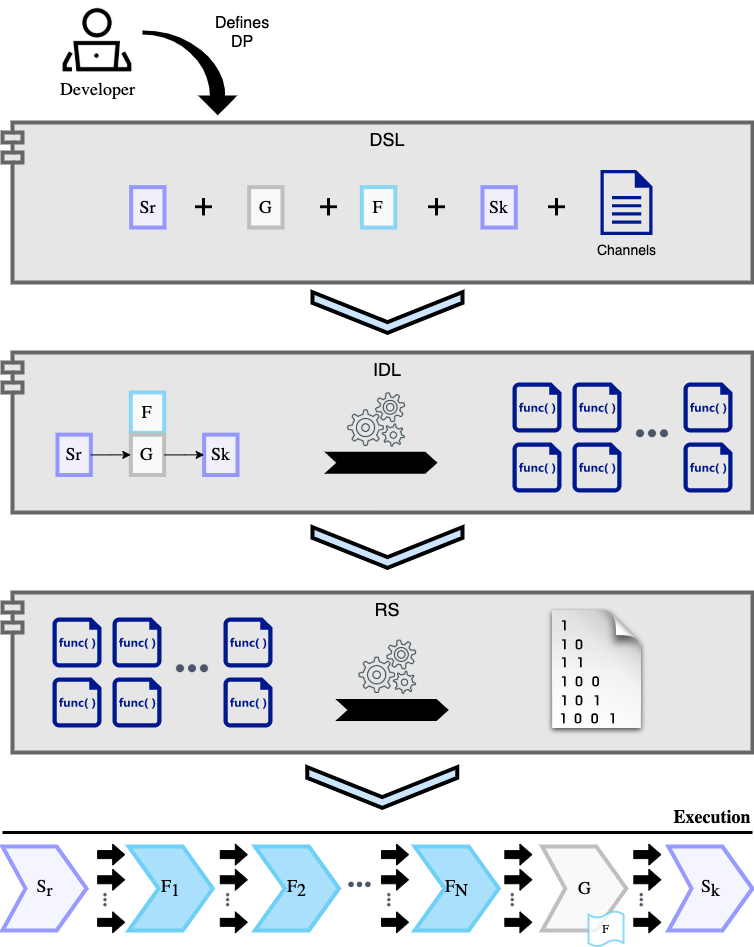
\includegraphics[width = 0.8\textwidth, height = 0.8\textheight]{dpf_haskell_v3}
    \end{center}
  \end{frame}

    \begin{frame}[fragile]{DP Framework: Haskell}
      \begin{center}
      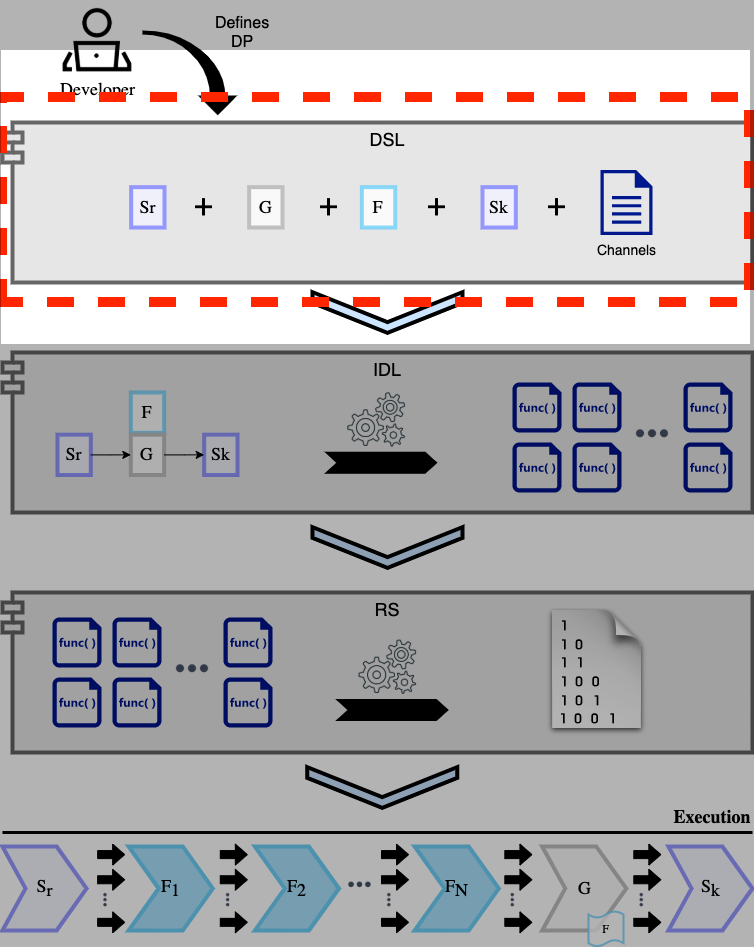
\includegraphics[width = 0.8\textwidth, height = 0.8\textheight]{dpf_haskell_v3-1}
    \end{center}
  \end{frame}

  \lstset{
    basicstyle=\itshape,
    literate={->}{$\rightarrow$}{2}
  }

  \begin{frame}[fragile]{DP Framework: Haskell}
    \frametitle{DSL Grammar}
    \small
    \begin{equation*}
      \boxed{
       \begin{aligned}
      G_{dsl} = (N, \Sigma, DB, P)
      \end{aligned}
      }
  \end{equation*}
  \tiny
      \begin{equation*}
          \boxed{
           \begin{aligned}
          N &= \{DP,S_r,S_k,G,F_b,CH,CH_s\},\\
          \Sigma &= \{\text{\mintinline{haskell}{Source}},\text{\mintinline{haskell}{Generator}},\text{\mintinline{haskell}{Sink}},\text{\mintinline{haskell}{FeedbackChannel}},\text{\mintinline{haskell}{Type}},\text{\mintinline{haskell}{Eof}},\text{\mintinline{haskell}{:=>}},\text{\mintinline{haskell}{:<+>}}\},
          \end{aligned}
          }
      \end{equation*}
    \small
    \begin{equation*}
      \boxed{
        \begin{aligned}
      P = \{\\
      DP  &\rightarrow S_r\ \text{\mintinline{haskell}{:=>}}\ G\ \text{\mintinline{haskell}{:=>}}\ S_k\ |\ S_r\ \text{\mintinline{haskell}{:=>}}\ G\ \text{\mintinline{haskell}{:=>}}\ F_b\ \text{\mintinline{haskell}{:=>}}\ S_k,\\
      S_r &\rightarrow \text{\mintinline{haskell}{Source}}\ CH_s,\\
      G   &\rightarrow \text{\mintinline{haskell}{Generator}}\ CH_s,\\
      S_k &\rightarrow \text{\mintinline{haskell}{Sink}},\\
      F_b &\rightarrow \text{\mintinline{haskell}{FeedbackChannel}} CH,\\
      CH_s &\rightarrow \text{\mintinline{haskell}{Channel}}\ CH,\\
      CH &\rightarrow \text{\mintinline{haskell}{Type :<+>}}\ CH\ |\ \text{\mintinline{haskell}{Eof}}\}
    \end{aligned}
    }
    \end{equation*}
  \end{frame}

  \begin{frame}[fragile]{DP Framework: Haskell}
    \begin{itemize}
      \item The specification of \textbf{DP} in the Language is compile time checked (\textit{Type-safe})
    \end{itemize}    
    \begin{exampleblock}{Type Level DSL}
      \begin{minted}[fontsize=\small,breaklines,highlightlines={7-17}]{shell}      
ghci> import DynamicPipeline
ghci> type DPExample = Source (Channel (Int :<+> Eof)) :=> Generator (Channel (Int :<+> Eof)) :=> Sink
type DPExample :: *
type DPExample =
  Source (Channel (Int :<+> Eof))
  :=> (Generator (Channel (Int :<+> Eof)) :=> Sink)
ghci> :t mkDP @DPExample
mkDP @DPExample
  :: forall k (st :: k) filterState filterParam.
      Stage (WriteChannel Int -> DP st ())
      -> GeneratorStage DPExample filterState filterParam st
      -> Stage (ReadChannel Int -> DP st ())
      -> DP st ()    
    \end{minted}
    \end{exampleblock}
  \end{frame}

  % \begin{frame}[fragile]{DP Framework: Haskell}
  %   \begin{itemize}
  %     \item Otherwise the compiler warns us about \textbf{Grammar Verification Error}
  %   \end{itemize}    
  % \end{frame}

%   \begin{frame}[fragile]{DP Framework: Haskell}
%     \begin{itemize}
%       \item Otherwise the compiler warns us about \textbf{Grammar Verification Error}
%     \end{itemize}    
%     \begin{alertblock}{Type Level DSL}
%     \begin{minted}[fontsize=\small,breaklines,highlightlines={8-17},highlightcolor=titaniumyellow]{shell}      
% ghci> type DPExample2 = Source (Channel Int) :=> Generator (Channel (Int :<+> Eof)) :=> Sink
% type DPExample2 :: *
% type DPExample2 =
%   Source (Channel Int)
%   :=> (Generator (Channel (Int :<+> Eof)) :=> Sink)
% ghci> :t mkDP @DPExample2

% <interactive>:1:1: error:
%     Invalid Semantic for Source Stage
%     in the DP Definition 'ChanIn Int'
%     Language Grammar:
%     DP       -> Source CHANS :=> Generator CHANS :=> Sink
%     DP       -> Source CHANS :=> Generator CHANS :=> FEEDBACK :=> Sink
%     CHANS    -> Channel CH
%     FEEDBACK -> FeedbackChannel CH
%     CH       -> Type :<+> CH | Eof
%     Example: 'Source (Channel (Int :<+> Int)) :=> Generator (Channel (Int :<+> Int)) :=> Sink'    
%     \end{minted}
%     \end{alertblock}
%   \end{frame}

  \begin{frame}[fragile]{DP Framework: Haskell}
    \begin{center}
      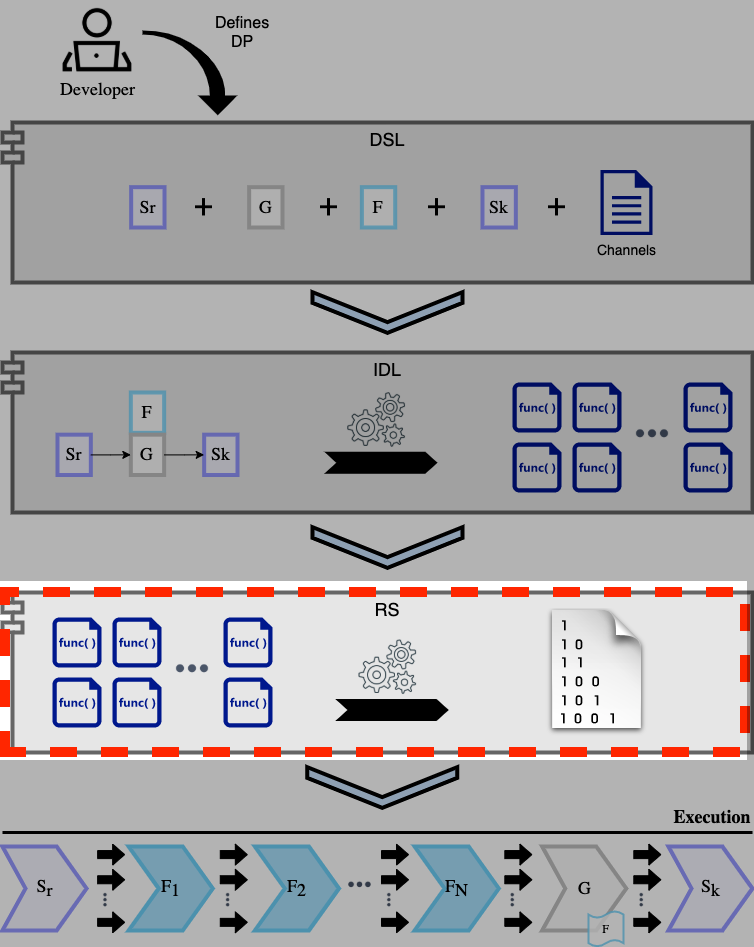
\includegraphics[width = 0.8\textwidth, height = 0.8\textheight]{dpf_haskell_v3-3}
    \end{center}
  \end{frame}

  \begin{frame}[fragile]{DP Framework: Haskell}
    \begin{block}{Runtime System}
      \begin{itemize}
        \item \textbf{DP Monad}:
        \begin{itemize} 
        \item Monad with Existential Type to not escape DP Context. (\textit{Rank-2 Polymorphic type})
        \item Associativity Monad law guarantees execution flow (\mintinline{haskell}{ source >>= generator >>= sink }) 
        \end{itemize}
      \end{itemize}
    \end{block}
    \end{frame}
  
  \begin{frame}[fragile]{DP Framework: Haskell}
    \begin{block}{Runtime System}
      \begin{itemize}
        \item \textbf{DP Monad}:
        \begin{itemize} 
        \item Monad with Existential Type to not escape DP Context. (\textit{Rank-2 Polymorphic type})
        \item Associativity Monad law guarantees execution flow (\mintinline{haskell}{ source >>= generator >>= sink }) 
        \end{itemize}
        \item \textbf{Filter / Stage}: 
        \begin{itemize}
          \item Use of \mintinline{haskell}{unfold} to generate dynamic filter computations (\textit{Anamorphism})
          \item Use of \mintinline{haskell}{fold} to reduce results to Sink (\textit{Catamorphism})
        \end{itemize}
      \end{itemize}
    \end{block}
    \end{frame}
  
  \begin{frame}[fragile]{DP Framework: Haskell}
    \begin{block}{Runtime System}
      \begin{itemize}
        \item \textbf{DP Monad}:
        \begin{itemize} 
        \item Monad with Existential Type to not escape DP Context. (\textit{Rank-2 Polymorphic type})
        \item Associativity Monad law guarantees execution flow (\mintinline{haskell}{ source >>= generator >>= sink }) 
        \end{itemize}
        \item \textbf{Filter / Stage}: 
        \begin{itemize}
          \item Use of \mintinline{haskell}{unfold} to generate dynamic filter computations (\textit{Anamorphism})
          \item Use of \mintinline{haskell}{fold} to reduce results to Sink (\textit{Catamorphism})
        \end{itemize}
        \item \textbf{Multithreading}: \mintinline{shell}{async} library
      \end{itemize}
    \end{block}
    \end{frame}
  
  \begin{frame}[fragile]{DP Framework: Haskell}
  \begin{block}{Runtime System}
    \begin{itemize}
      \item \textbf{DP Monad}:
      \begin{itemize} 
      \item Monad with Existential Type to not escape DP Context. (\textit{Rank-2 Polymorphic type})
      \item Associativity Monad law guarantees execution flow (\mintinline{haskell}{ source >>= generator >>= sink }) 
      \end{itemize}
    \item \textbf{Filter / Stage}: 
      \begin{itemize}
        \item Use of \mintinline{haskell}{unfold} to generate dynamic filter computations (\textit{Anamorphism})
        \item Use of \mintinline{haskell}{fold} to reduce results to Sink (\textit{Catamorphism})
      \end{itemize}
      \item \textbf{Multithreading}: \mintinline{shell}{async} library
      \item \textbf{Channels}: \mintinline{shell}{unagi-chan} library
    \end{itemize}
  \end{block}
  \end{frame}

  \begin{frame}[fragile]{DP Framework: Haskell}
    \begin{center}
      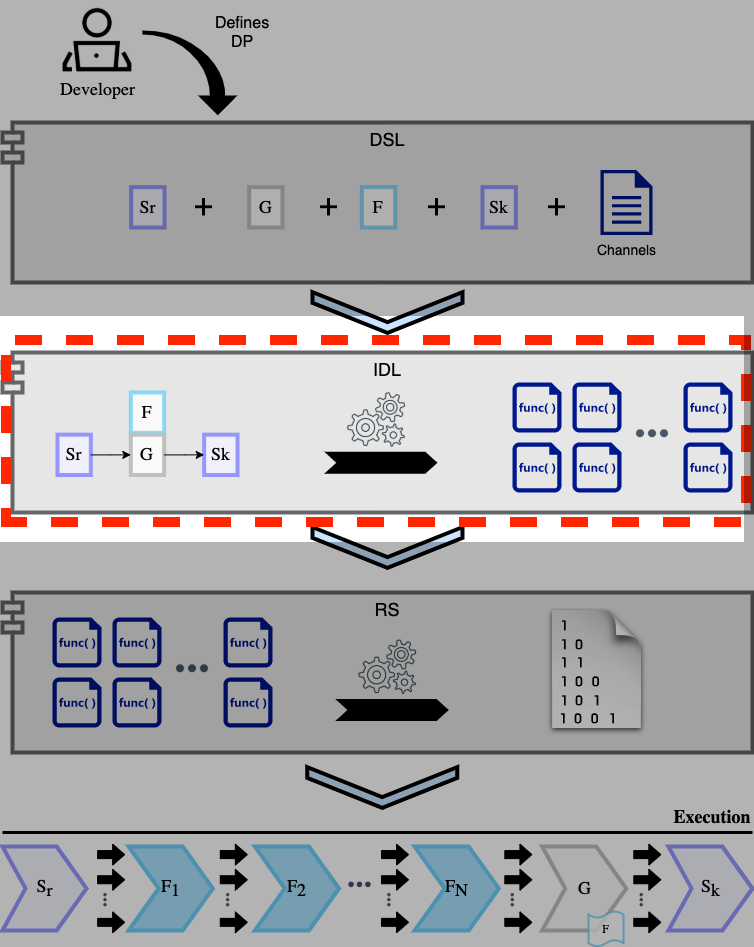
\includegraphics[width = 0.8\textwidth, height = 0.8\textheight]{dpf_haskell_v3-2}
    \end{center}
  \end{frame}

  \begin{frame}[fragile]{DP Framework: Haskell}
    \begin{block}{IDL}
      \begin{minted}[fontsize=\small,breaklines]{shell}      
ghci> type DPExample = Source (Channel (Int :<+> Eof)) :=> Generator (Channel (Int :<+> Eof)) :=> Sink
type DPExample :: *
type DPExample =
  Source (Channel (Int :<+> Eof))
  :=> (Generator (Channel (Int :<+> Eof)) :=> Sink)
    \end{minted}
  \end{block}
  \end{frame}

  \begin{frame}[fragile]{DP Framework: Haskell}
    \begin{block}{IDL}
      \begin{minted}[fontsize=\small,breaklines,highlightlines={7-11}]{shell}      
ghci> type DPExample = Source (Channel (Int :<+> Eof)) :=> Generator (Channel (Int :<+> Eof)) :=> Sink
type DPExample :: *
type DPExample =
  Source (Channel (Int :<+> Eof))
  :=> (Generator (Channel (Int :<+> Eof)) :=> Sink)
        
ghci> :t withSource @DPExample
withSource @DPExample
  :: forall k (st :: k).
      (WriteChannel Int -> DP st ())
      -> Stage (WriteChannel Int -> DP st ())
    \end{minted}
  \end{block}
  \end{frame}

  \begin{frame}[fragile]{DP Framework: Haskell}
    \begin{block}{IDL}
      \begin{minted}[fontsize=\small,breaklines,highlightlines={7-9}]{shell}      
ghci> :t withSource @DPExample
withSource @DPExample
  :: forall k (st :: k).
      (WriteChannel Int -> DP st ())
      -> Stage (WriteChannel Int -> DP st ())
      
ghci> let source' = withSource @DPExample  $ \wc -> unfoldT ([1..10] <> [1..10]) wc identity
ghci> :t source'
source' :: forall k (st :: k). Stage (WriteChannel Int -> DP st ())
    \end{minted}
  \end{block}
  \end{frame}

  \begin{frame}[fragile]{DP Framework: Haskell}
    \begin{block}{IDL}
      \begin{minted}[fontsize=\small,breaklines,highlightlines={2-8}]{shell}      
ghci> :t withGenerator @DPExample
withGenerator @DPExample
  :: forall k filter (st :: k).
      (filter -> ReadChannel Int -> WriteChannel Int -> DP st ())
      -> Stage
          (filter -> ReadChannel Int -> WriteChannel Int -> DP st ())    
    \end{minted}
  \end{block}
  \end{frame}

  \begin{frame}[fragile]{DP Framework: Haskell}
    \begin{block}{IDL}
      \begin{minted}[fontsize=\small,breaklines,highlightlines={2-8}]{shell}      
ghci> :t withGenerator @DPExample
withGenerator @DPExample
  :: forall k filter (st :: k).
      (filter -> ReadChannel Int -> WriteChannel Int -> DP st ())
      -> Stage
          (filter -> ReadChannel Int -> WriteChannel Int -> DP st ())    
    \end{minted}
  \end{block}
  \begin{block}{Techniques}
    \begin{itemize}
      \item First Class Families
      \item Type-level Defunctionalization 
      \item Defunctionalization
      \item Associated Type Families
    \end{itemize}
  \end{block}
  \end{frame}

  \begin{frame}[fragile]{DP Framework: Haskell}
    \begin{block}{}
      Library released on Hackage \\
      https://hackage.haskell.org/package/dynamic-pipeline
      \begin{center}
        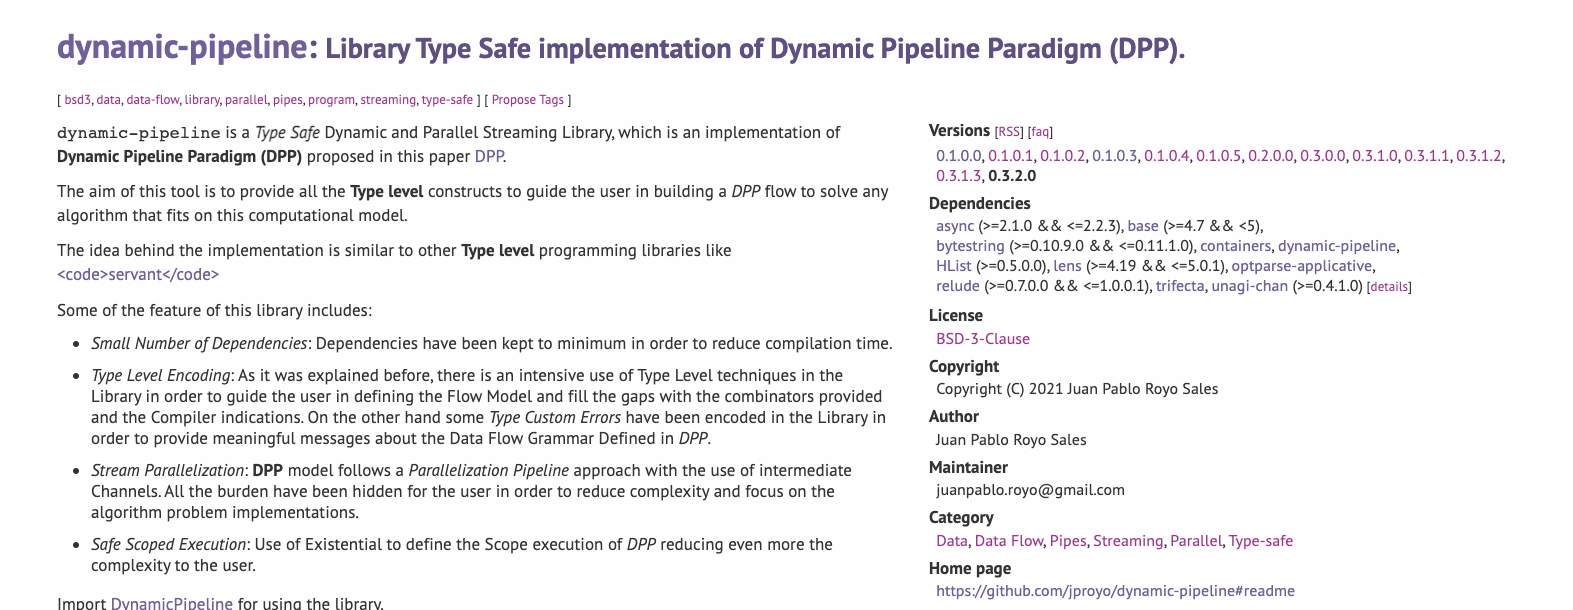
\includegraphics[width = 0.9\textwidth, height = 0.6\textheight]{dp-fw-hs}
      \end{center}  
    \end{block}
  \end{frame}

  \begin{frame}{Agenda}
    \section{$DP_{WCC}$: Computing $WCC$}
    \tableofcontents[currentsection]
  \end{frame}

  \begin{frame}[fragile]{$DP_{WCC}$: Computing $WCC$}
    \begin{block}{Program}
      \begin{minted}[fontsize=\small,breaklines,highlightlines={5-6}]{haskell}      
type DPConnComp = Source (Channel (Edge :<+> ConnectedComponents :<+> Eof))
:=> Generator (Channel (Edge :<+> ConnectedComponents :<+> Eof))
:=> Sink

program :: FilePath -> IO ()
program file = runDP $ mkDP @DPConnComp (source' file) generator' sink'
      \end{minted}
    \end{block}
  \end{frame}


  \begin{frame}[fragile]{$DP_{WCC}$: Computing $WCC$}
    \begin{block}{Program}
      \begin{minted}[fontsize=\small,breaklines,highlightlines={5-9}]{haskell}      
type DPConnComp = Source (Channel (Edge :<+> ConnectedComponents :<+> Eof))
:=> Generator (Channel (Edge :<+> ConnectedComponents :<+> Eof))
:=> Sink

source' :: FilePath
        -> Stage
           (WriteChannel Edge -> WriteChannel ConnectedComponents -> DP st ())
source' filePath = withSource @DPConnComp
  $ \edgeOut _ -> unfoldFile filePath edgeOut (toEdge . decodeUtf8)

program :: FilePath -> IO ()
program file = runDP $ mkDP @DPConnComp (source' file) generator' sink'  
      \end{minted}
    \end{block}
  \end{frame}

  \begin{frame}[fragile]{$DP_{WCC}$: Computing $WCC$}
    \begin{block}{Program}
      \begin{minted}[fontsize=\small,breaklines,highlightlines={5-7}]{haskell}      
type DPConnComp = Source (Channel (Edge :<+> ConnectedComponents :<+> Eof))
:=> Generator (Channel (Edge :<+> ConnectedComponents :<+> Eof))
:=> Sink

sink' :: Stage (ReadChannel Edge -> ReadChannel ConnectedComponents -> DP st ())
sink' = withSink @DPConnComp $ \_ cc -> withDP $ foldM_ cc print

program :: FilePath -> IO ()
program file = runDP $ mkDP @DPConnComp (source' file) generator' sink'  
      \end{minted}
    \end{block}
  \end{frame}

  \begin{frame}[fragile]{$DP_{WCC}$: Computing $WCC$}
    \begin{block}{Program}
      \begin{minted}[fontsize=\small,breaklines,highlightlines={7-8,11-11}]{haskell}      
type DPConnComp = Source (Channel (Edge :<+> ConnectedComponents :<+> Eof))
:=> Generator (Channel (Edge :<+> ConnectedComponents :<+> Eof))
:=> Sink

generator' :: GeneratorStage DPConnComp ConnectedComponents Edge st
generator' =
  let gen = withGenerator @DPConnComp genAction
  in  mkGenerator gen filterTemplate

filterTemplate :: Filter DPConnComp ConnectedComponents Edge st
filterTemplate = actor actor1 |>> actor actor2

program :: FilePath -> IO ()
program file = runDP $ mkDP @DPConnComp (source' file) generator' sink'
      \end{minted}
    \end{block}
  \end{frame}

  \begin{frame}[fragile]{$DP_{WCC}$: Computing $WCC$}
    \begin{block}{Program}
      \begin{minted}[fontsize=\small,breaklines,highlightlines={11-14}]{haskell}      
type DPConnComp = Source (Channel (Edge :<+> ConnectedComponents :<+> Eof))
:=> Generator (Channel (Edge :<+> ConnectedComponents :<+> Eof))
:=> Sink

genAction :: Filter DPConnComp ConnectedComponents Edge st
          -> ReadChannel Edge
          -> ReadChannel ConnectedComponents
          -> WriteChannel Edge
          -> WriteChannel ConnectedComponents
          -> DP st ()
genAction filter' readEdge readCC _ writeCC = do
  let unfoldFilter = mkUnfoldFilterForAll filter' toConnectedComp readEdge (readCC .*. HNil) 
  results <- unfoldF unfoldFilter
  foldM_ (hHead results) (`push` writeCC)
      \end{minted}
    \end{block}
  \end{frame}

  \begin{frame}[fragile]{$DP_{WCC}$: Computing $WCC$}
    \begin{block}{Program}
      \begin{minted}[fontsize=\tiny,breaklines,highlightlines={7-12,20-28}]{haskell}      
actor1 :: Edge
       -> ReadChannel Edge
       -> ReadChannel ConnectedComponents
       -> WriteChannel Edge
       -> WriteChannel ConnectedComponents
       -> StateT ConnectedComponents (DP st) ()
actor1 _ readEdge _ writeEdge _ = 
  foldM_ readEdge $ \e -> get >>= doActor e
 where
  doActor v conn
    | toConnectedComp v `intersect` conn = modify (toConnectedComp v <>)
    | otherwise = push v writeEdge

actor2 :: Edge
       -> ReadChannel Edge
       -> ReadChannel ConnectedComponents
       -> WriteChannel Edge
       -> WriteChannel ConnectedComponents
       -> StateT ConnectedComponents (DP st) ()
actor2 _ _ readCC _ writeCC = do 
  foldWithM_ readCC pushMemory $ \e -> get >>= doActor e

 where
   pushMemory = get >>= flip push writeCC

   doActor cc conn
    | cc `intersect` conn = modify (cc <>)
    | otherwise = push cc writeCC
      \end{minted}
    \end{block}
  \end{frame}

  \begin{frame}{Agenda}
    \section{Empirical Evaluation}
    \tableofcontents[currentsection]
  \end{frame}


  \begin{frame}[fragile]{Empirical Evaluation}
    \begin{block}{Research Questions}
      \begin{itemize}
            \item Does $\dpwcc$ in Haskell support the dynamic parallelization level that $\dpwcc$ requires?
            \item Is $\dpwcc$ in Haskell competitive compared with default implementations on base libraries for the same problem?
            \item Does $\dpwcc$ in Haskell handle memory efficiently?
        \end{itemize}        
    \end{block}
    \begin{block}{Experiments}
      \begin{itemize}
        \item \textbf{Implementation Analysis}: Measure and analyze Total execution time, MUT time and GC Time.
        \item \textbf{Benchmark Analysis}: Compare $DP_{WCC}$ with \mintinline{haskell}{Data.Graph} $WCC$ execution times:
        \begin{itemize}
          \item Using \mintinline{haskell}{ criterion } library.
          \item Diefficency metric $\mathtt{dief@t}$ (\textit{diepfy} tool) to measure incremental results.
        \end{itemize}
        \item \textbf{Performance Analysis}: Thread and Memory allocation analysis.
      \end{itemize}
    \end{block}
  \end{frame}

  \begin{frame}[fragile]{Empirical Evaluation}
    \begin{block}{Graphs Tested}
    \begin{table}[H]
      \centering
      \begin{tabular}{|p{0.25\linewidth}|r|r|r|p{0.25\linewidth}|}
       \hline
       \textbf{Network} & \textbf{Nodes} & \textbf{Edges} & \textbf{\#WCC} & \textbf{\#Nodes Largest WCC} \\
       \hline
       Enron Emails & 36692 & 183831 & 1065 & 33696 (0.918) \\
       \hline
       Astro Physics Collaboration Net & 18772 & 198110 & 290 & 17903 (0.954)\\
       \hline
       Google Web Graph & 875713 & 5105039 & 2746 & 855802 (0.977)\\
       \hline
      \end{tabular}
     \end{table}
    \end{block}
    \begin{block}{Hardware Environment}
      \begin{itemize}
            \item $x86$ $64$ bits
            \item $6$-Core Intel Core i7 processor of $2,2$ GHz up to $12$ virtual cores
            \item \emph{Hyper-threading} enable
            \item $32 GB$ \emph{DDR4} of RAM, $256\ KB$ of L2 cache memory, and $9\ MB$ of L3 cache
        \end{itemize}        
    \end{block}
  \end{frame}

  \begin{frame}[fragile]{Empirical Evaluation}
    \frametitle{Diefficiency Metrics}
      \begin{figure}[!htb]
        \centering
        \begin{minipage}{0.33\textwidth}
         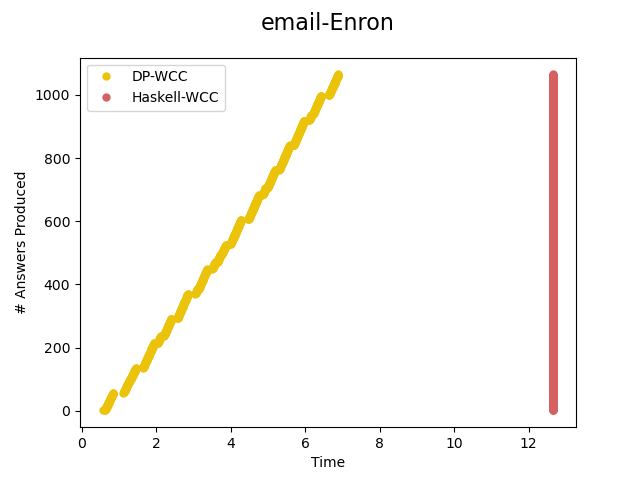
\includegraphics[width=1\linewidth, height=0.4\textheight]{email_enron}
        \end{minipage}%
        \begin{minipage}{0.33\textwidth}
         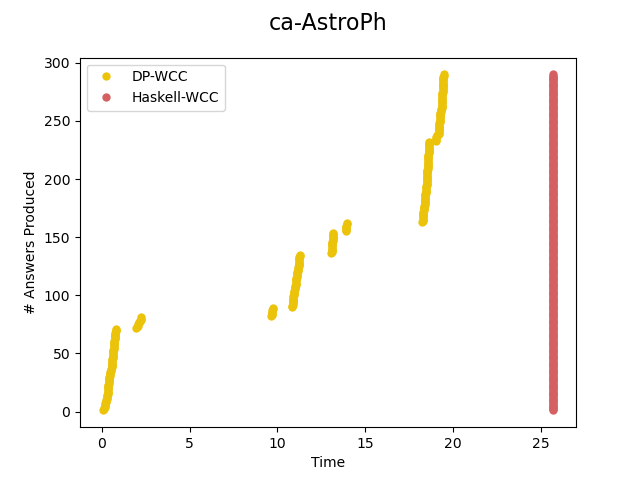
\includegraphics[width=1\linewidth, height=0.4\textheight]{ca_astroph}
        \end{minipage}%
        \begin{minipage}{0.33\textwidth}
         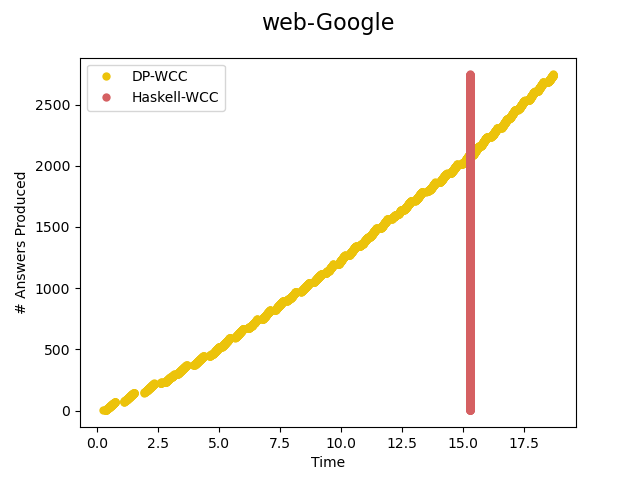
\includegraphics[width=1\linewidth, height=0.4\textheight]{web_google}
        \end{minipage}
    \end{figure}
  \begin{figure}[!htb]
      \centering
      \begin{minipage}{0.33\textwidth}
       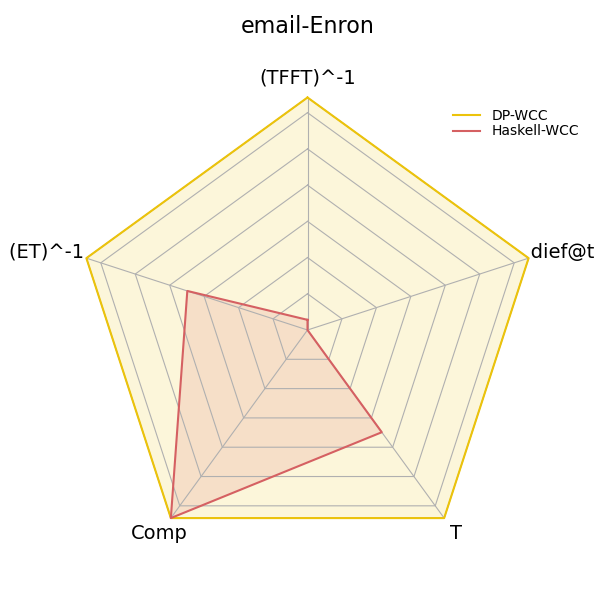
\includegraphics[width=1\linewidth, height=0.35\textheight]{email_enron_radar}
      \end{minipage}%
      \begin{minipage}{0.33\textwidth}
       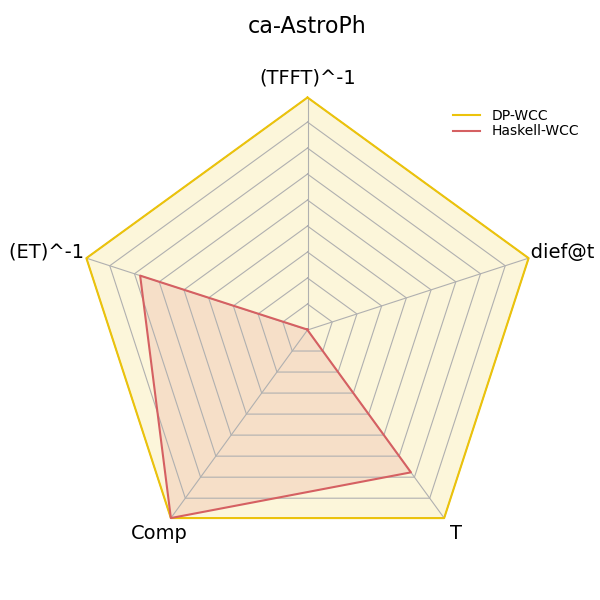
\includegraphics[width=1\linewidth, height=0.35\textheight]{ca_astroph_radar}
      \end{minipage}%
      \begin{minipage}{0.33\textwidth}
       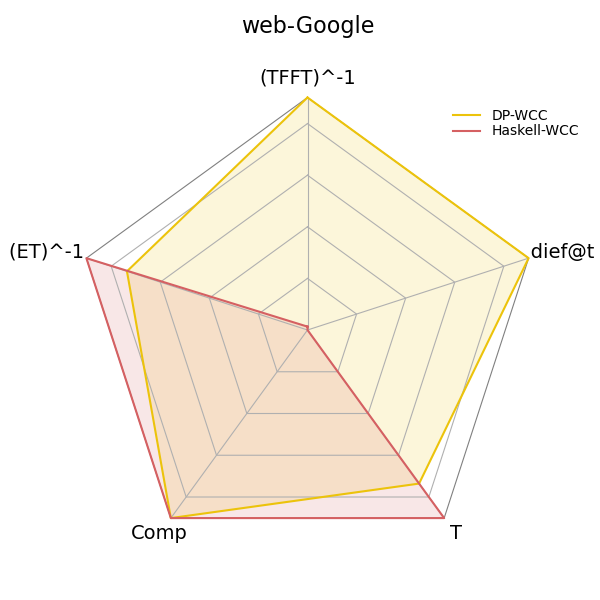
\includegraphics[width=1\linewidth, height=0.35\textheight]{web_google_radar}
      \end{minipage}
  \end{figure}
  \end{frame}

  \begin{frame}[fragile]{Empirical Evaluation}
    \frametitle{Benchmark}

    \begin{block}{Execution time}
    \begin{table}[H]
      \centering
      \begin{tabular}{|l|l|l|l|}
       \hline
       \textbf{Network} & \textbf{DP-Haskell} & \textbf{Data.Graph} & \textbf{Speed-up}\\
       \hline
       Enron Emails & 4.68s &  6.46s & 1.38\\
       \hline
       Astro Physics Coll Net & 4.98s & 6.95s  & 1.39\\
       \hline
       Google Web Graph & 386s & 106s & \color{red}0.27\\
       \hline
      \end{tabular}
     \end{table}      
    \end{block}

     \vspace{1cm}

    \begin{minipage}[t]{\linewidth}
      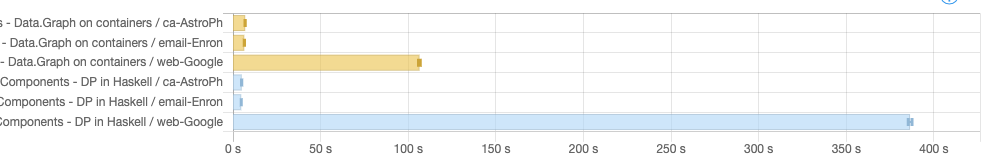
\includegraphics[width=\textwidth]{bench_2}
    \end{minipage}
  \end{frame}

  \begin{frame}[fragile]{Empirical Evaluation}
    \begin{columns}[onlytextwidth] 
      \begin{column}{.45\textwidth} 
        \begin{block}{ThreadScope}
          \begin{minipage}{\textwidth}
            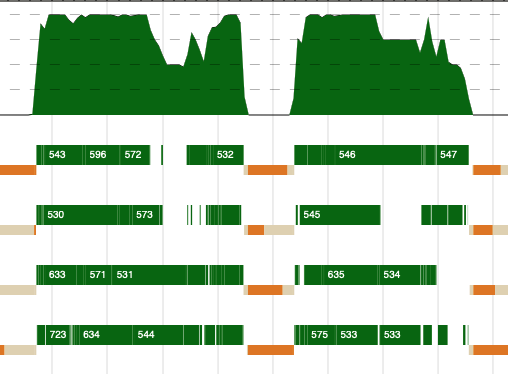
\includegraphics[width=1\linewidth, height=0.5\textheight]{screen_2}
          \end{minipage}%     
        \end{block}%
      \end{column} \hfill%
      \begin{column}{.45\textwidth} 
        \begin{block}{Eventlog - Memory Allocation}
          \begin{minipage}{\textwidth}
            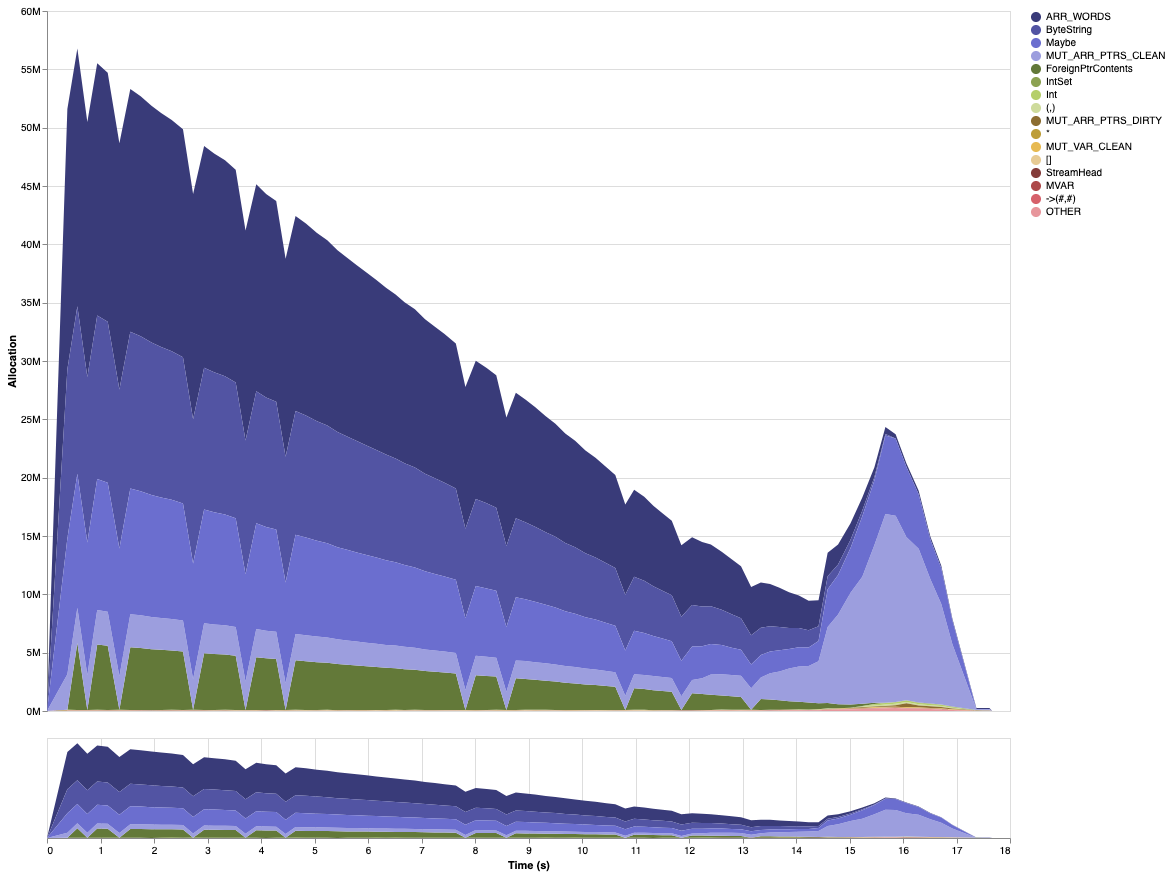
\includegraphics[width=1\linewidth, height=0.5\textheight]{visualization}
          \end{minipage}%
        \end{block}
    \end{column} 
  \end{columns}
  \end{frame}

  \begin{frame}{Agenda}
    \section{Conclusions and Future Work}
    \tableofcontents[currentsection]
  \end{frame}

  \begin{frame}[fragile]{Conclusions and Future Work}
    \begin{block}{Conclusions}      
      \begin{itemize}
        \item \textbf{Robustness and Suitability} of the DP-Haskell 
      \end{itemize}
    \end{block}
  \end{frame}

  \begin{frame}[fragile]{Conclusions and Future Work}
    \begin{block}{Conclusions}      

    \begin{itemize}
      \item \textbf{Robustness and Suitability} of the DP-Haskell 
      \item \textbf{Ability to generate Incremental results} has been shown by $\mathtt{dief@t}$ metrics 
    \end{itemize}
  \end{block}
  \end{frame}

  \begin{frame}[fragile]{Conclusions and Future Work}
    \begin{block}{Conclusions}      

    \begin{itemize}
      \item \textbf{Robustness and Suitability} of the DP-Haskell 
      \item \textbf{Ability to generate Incremental results} has been shown by $\mathtt{dief@t}$ metrics
      \item \textbf{Satisfactory Performance results} with an adequate Memory allocation and Execution times. 
    \end{itemize}
  \end{block}
  \end{frame}

  \begin{frame}[fragile]{Conclusions and Future Work}
    \begin{block}{Future work}      
    \begin{itemize}
      \item \textbf{Explore other Algorithms} to be implemented with this Paradigm.\footnote{We are currently working on Bi-partite Graphs algorithms}
      \item \textbf{Improve DP Framework} implementing more combinators and abstractions to allow the user write better and faster programs.
    \end{itemize}
  \end{block}
  \end{frame}

  \begin{frame}
    \centering \Huge
    \emph{Questions?}
  \end{frame}  
  
\end{document}